% !TEX program = pdflatex
\documentclass[letterpaper,12pt]{article}
\usepackage[spanish,mexico]{babel}
\usepackage[T1]{fontenc}
\usepackage{lmodern}
\usepackage{amsmath,amssymb}
\usepackage{graphicx,float,subcaption,xcolor,array,booktabs,tabularx,ragged2e}
\usepackage{tikz}
\usetikzlibrary{positioning,arrows.meta,calc,shapes.geometric}
\usepackage{listings}
\usepackage{pdflscape}
\usepackage[left=25mm,right=25mm,top=35mm,bottom=30mm,headheight=15pt]{geometry}
\usepackage{parskip,fancyhdr}
\usepackage{hyperref}

\graphicspath{{img/}{portada_img/}}
\newcommand{\materia}{Laboratorio de Organización y Arquitectura de Computadoras}
\pagestyle{fancy}
\fancyhf{}
\fancyhead[R]{\textsc{\materia}}
\fancyfoot[C]{\thepage}
\renewcommand{\headrulewidth}{0.8pt}
\hypersetup{colorlinks=true,linkcolor=blue,urlcolor=cyan}

\definecolor{codebg}{rgb}{0.96,0.96,0.96}
\definecolor{keyword}{rgb}{0.0,0.2,0.6}
\definecolor{comment}{rgb}{0.25,0.5,0.35}
\definecolor{codegray}{rgb}{0.5,0.5,0.5}
\lstdefinestyle{estiloVHDL}{
  language=VHDL,basicstyle=\ttfamily\scriptsize,
  backgroundcolor=\color{codebg},commentstyle=\color{comment}\itshape,
  keywordstyle=\color{keyword}\bfseries,numbers=left,
  numberstyle=\tiny\color{codegray},frame=single,breaklines=true,
  literate={á}{{\'a}}1 {é}{{\'e}}1 {í}{{\'i}}1 {ó}{{\'o}}1 {ú}{{\'u}}1 {ñ}{{\~n}}1,
  keepspaces=true,showstringspaces=false,tabsize=4,
  morekeywords={library,use,all,entity,is,port,in,out,architecture,of,begin,end,signal,constant,process,if,then,else,elsif,case,when,others,std_logic,std_logic_vector}
}

\begin{document}
\thispagestyle{empty} % Sin encabezado ni pie en la portada

% --- ENCABEZADO DE PORTADA (TABLA DE 3 COLUMNAS) ---
\begin{center}
    % La tabla usa 'm' para centrar verticalmente las imágenes y el texto
    \begin{tabular}{m{0.15\textwidth} m{0.60\textwidth} m{0.15\textwidth}}
        % Logo Izquierdo (UNAM)
        
\includegraphics[width=2cm]{portada_img/escudounam_negro.jpg} & 
        
        % Título Central
        \centering\Huge\textbf{Universidad Nacional Autónoma de México} &
        
        % Logo Derecho (Facultad)
        \raggedleft
\includegraphics[width=2cm]{portada_img/escudofi_negro.jpg}
    \end{tabular}
\end{center}

\vspace{0.3cm}

% --- INFORMACIÓN DEL REPORTE ---
\begin{center}
    {\LARGE \textbf{Facultad de Ingeniería}}\\[1cm]

    {\LARGE \textbf{Laboratorio de Arquitectura y Organización de Computadoras}} \\[1cm]

	{\LARGE Grupo: 07 - Semestre: 2027-1} \\[1cm]
    
    {\LARGE \textbf{Reporte Practica 3}}\\[0.5cm]
    {\LARGE {Construción de M´aquinas de estados Usando Memorias Direccionamiento por Trayectoria}}\\[1cm]

    {\Large \textbf{Fecha de Entrega}}\\[0.2cm]
    {\Large 25 de Septiembre del 2026} \\[1cm]

    {\LARGE \textbf{Profesor}}\\[0.2cm]
    {\Large Ing. Julio Cesar Cruz Estrada}\\[1cm]
    
    {\LARGE \textbf{Integrantes:}}\\[0.2cm]
    {\Large Espinoza Matamoros Percival Ulises}\\[0.5cm]
    {\Large Montiel Juárez Oscar Iván}\\[0.5cm]
    {\Large Veraza García Amy Valentina}\\[0.5cm]

\end{center}
\newpage

\section{Objetivo}

Familiarizar al alumno en el conocimiento de construcción de máquinas de estados usando direccionamiento de memorias con el método de direccionamiento entrada-estado.

\section{Desarrollo}

El método de direccionamiento entrada-estado se aplica a cartas ASM en las que cada estado consulta una sola variable de entrada. A diferencia del direccionamiento por trayectoria, la dirección de la ROM depende únicamente del estado presente. La palabra almacenada contiene el código de la entrada que debe probarse, dos ligas posibles y dos conjuntos de salidas. Un selector de entrada obtiene el valor de la variable indicada con dicho valor, los selectores de liga y de salida escogen la alternativa falsa o verdadera.

Para esta práctica se implementó la carta ASM propia mostrada en la Figura[\ref{fig:carta-asm}]. Las entradas se denominaron $A$, $B$ y $C$, y las salidas se representaron por $S_3S_2S_1S_0$. La máquina tiene seis estados útiles, codificados de $000$ a $101$. El registro mantiene el estado presente y lo usa directamente como dirección de la ROM por ello, cada estado requiere una única palabra de memoria.

\subsection{Carta ASM y asignaciones binarias}

La carta ASM se diseñó con tres condicionales: en $S_0$ se evalúa $A$, en $S_1$ se evalúa $B$ y en $S_2$ se evalúa $C$. Los estados $S_3$, $S_4$ y $S_5$ no dependen de una entrada, por lo que su transición se fuerza al colocar las mismas ligas y salidas en las alternativas falsa y verdadera. De esta forma el valor seleccionado no modifica el resultado.

\begin{figure}[H]
\centering
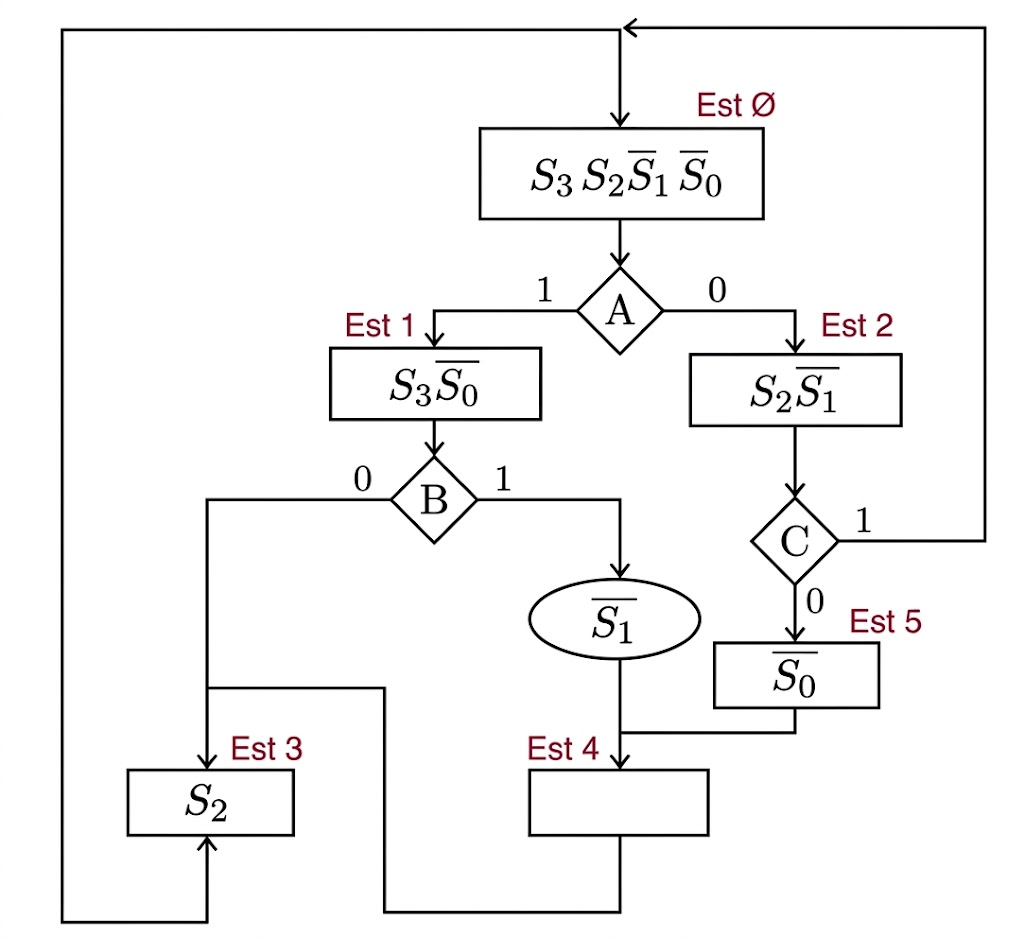
\includegraphics[width=0.84\linewidth]{carta_asm.jpeg}
\caption{Carta ASM propia utilizada para el direccionamiento entrada-estado.}
\label{fig:carta-asm}
\end{figure}

La asignación binaria de estados y de entradas es la siguiente:
\[
\begin{array}{c|cccccc}
\text{Estado} & S_0 & S_1 & S_2 & S_3 & S_4 & S_5\\ \hline
Q_2Q_1Q_0 & 000 & 001 & 010 & 011 & 100 & 101
\end{array}
\qquad
\begin{array}{c|ccc}
\text{Entrada} & A & B & C\\ \hline
P_1P_0 & 00 & 01 & 10
\end{array}
\]
El código \texttt{11} de prueba queda disponible como valor auxiliar: en \texttt{mux\_prueba.vhd} se implementa como cero. En los estados sin decisión, la implementación utiliza \texttt{00}, pero como sus campos falso y verdadero son idénticos, el selector es indiferente para la transición y las salidas.

\subsection{Dimensionamiento de la memoria}

Se requieren \texttt{3} bits para codificar los seis estados. Puesto que la dirección se forma sólo con el estado presente, la ROM tiene \texttt{3} bits de dirección. La palabra de memoria se divide en cinco campos:
\[
\underbrace{P_1P_0}_{2\ \text{bits de prueba}}\;
\underbrace{LF_2 \, LF_1 \,LF_0}_{3\ \text{bits de liga falsa}}\;
\underbrace{LV_2 \, LV_1 \,LV_0}_{3\ \text{bits de liga verdadera}}\;
\underbrace{SF_3 \, SF_2 \, SF_1 \,SF_0}_{4\ \text{salidas falsas}}\;
\underbrace{SV_3 \, SV_2 \, SV_1 \,SV_0}_{4\ \text{salidas verdaderas}}.
\]
Por tanto,
\[
m=2+3+3+4+4=16\ \text{bits},
\qquad
\text{ROM}=2^n\times m=2^3\times16=8\times16\ \text{bits}.
\]
La capacidad total requerida es de \texttt{128} bits. Las dos direcciones no utilizadas por los seis estados de la carta, \texttt{110} y \texttt{111}, se programaron como recuperación segura hacia $S_0$, con salidas \texttt{0011}.

\subsection{Contenido de la memoria}

La Tabla[\ref{tab:memoria}] contiene la palabra de memoria de cada estado. $P$ identifica la entrada que revisa \texttt{mux\_prueba}, $LF$ y $LV$ son las ligas que se seleccionan para $Qsel=0$ y $Qsel=1$, respectivamente. De la misma forma, $SF$ y $SV$ son las salidas para cada alternativa.

\begin{table}[H]
\centering
\small
\caption{Tabla de direccionamiento entrada-estado y contenido de la ROM.}
\label{tab:memoria}
\begin{tabular}{c c c c c c c}
\toprule
Estado & $Q_2Q_1Q_0$ & Prueba $P_1P_0$ & $LF$ & $LV$ & $SF$ & $SV$\\
\midrule
$S_0$ & 000 & 00 & 010 & 001 & 1100 & 1100\\
$S_1$ & 001 & 01 & 011 & 100 & 1010 & 1000\\
$S_2$ & 010 & 10 & 101 & 000 & 0101 & 0101\\
$S_3$ & 011 & $*$ & 000 & 000 & 0111 & 0111\\
$S_4$ & 100 & $*$ & 011 & 011 & 0011 & 0011\\
$S_5$ & 101 & $*$ & 100 & 100 & 0010 & 0010\\
No definidas & 110, 111 & $*$ & 000 & 000 & 0011 & 0011\\
\bottomrule
\end{tabular}
\end{table}

Por ejemplo, cuando el registro presenta \texttt{001}, la ROM entrega \texttt{01 011 100 1010 1000}. El selector de prueba interpreta \texttt{01} como la entrada $B$. Si $B=0$, la máquina avanza a \texttt{011} y presenta \texttt{1010}; si $B=1$, avanza a \texttt{100} y presenta \texttt{1000}. Esta sola palabra reemplaza las dos localidades que habría requerido el direccionamiento por trayectoria.

\subsection{Arquitectura e implementación en VHDL}

Las Figuras[\ref{fig:bloques-1}] y [\ref{fig:bloques-2}] muestran las capturas del diagrama de bloques implementado en Quartus. El estado presente se registra en cada flanco de reloj y direcciona la ROM. El bloque \texttt{div\_datos} separa los cinco campos de la palabra, \texttt{mux\_prueba} evalúa la entrada seleccionada y genera \texttt{Qsel}. Finalmente, \texttt{mux\_liga} y \texttt{mux\_salidas} escogen, con la misma señal, la liga y las salidas que corresponden a la decisión de la carta ASM.

\begin{figure}[H]
\centering
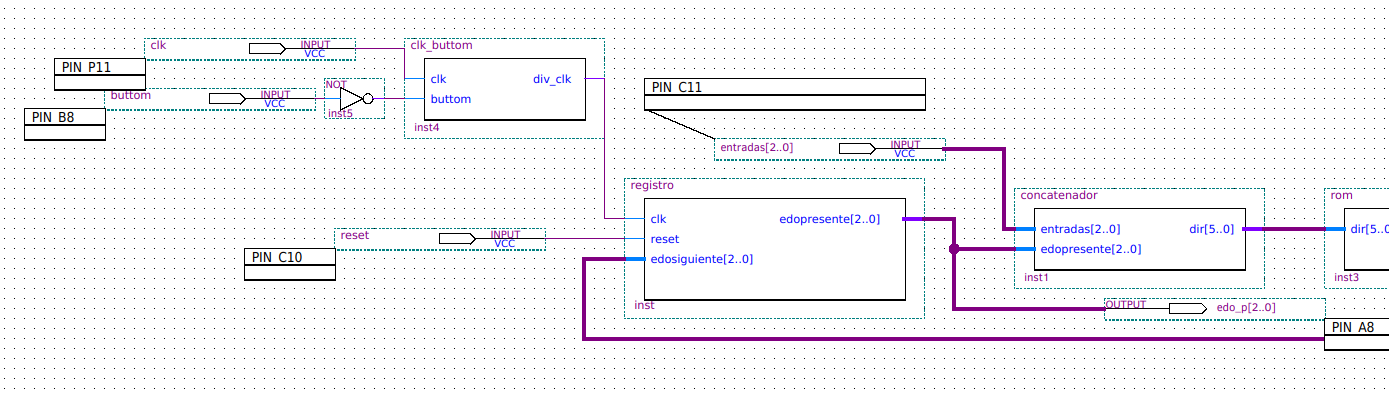
\includegraphics[width=\linewidth]{diagramas_bloques_1.png}
\caption{Primera parte del diagrama de bloques implementado en Quartus.}
\label{fig:bloques-1}
\end{figure}

\begin{figure}[H]
\centering
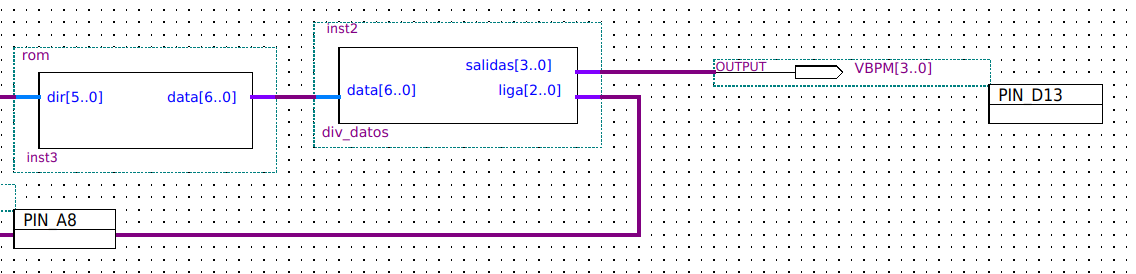
\includegraphics[width=0.92\linewidth]{diagramas_bloques_2.png}
\caption{Segunda parte del diagrama de bloques implementado en Quartus.}
\label{fig:bloques-2}
\end{figure}

\subsection{Módulos implementados}
Para los módulos implementados se reutilizaron los de la práctica anterior, el funcionamiento de cada uno de los módulos es el siguiente:

\paragraph{Registro:} El módulo \texttt{registro} almacena la liga seleccionada. Su reinicio es activo en bajo, donde si \texttt{reset='0'}, fuerza el estado \texttt{000}, por otro lado cuando \texttt{reset='1'}, actualiza el estado sólo en el flanco ascendente de \texttt{clk}. Esto asegura que cada transición de la máquina ocurra de manera síncrona.

\lstinputlisting[style=estiloVHDL,caption={Registro del estado presente.},label={lst:registro}]{code/registro.vhd}

\paragraph{ROM y división de datos:} \texttt{rom.vhd} declara ocho palabras de 16 bits y usa el estado presente como dirección. \texttt{div\_datos.vhd} no requiere reloj: separa los bits $[15:14]$ como prueba, $[13:11]$ como liga falsa, $[10:8]$ como liga verdadera, $[7:4]$ como salida falsa y $[3:0]$ como salida verdadera.

\lstinputlisting[style=estiloVHDL,caption={ROM de ocho palabras para el método entrada-estado.},label={lst:rom}]{code/rom.vhd}

\lstinputlisting[style=estiloVHDL,caption={Separación de los campos de la palabra de 16 bits.},label={lst:div-datos}]{code/div_datos.vhd}

\paragraph{Selección de entrada, liga y salidas.} \texttt{mux\_prueba} traduce los códigos \texttt{00}, \texttt{01} y \texttt{10} a $A$, $B$ y $C$. El resultado \texttt{Qsel} alimenta simultáneamente a \texttt{mux\_liga} y \texttt{mux\_salidas}: con cero se seleccionan $LF$ y $SF$; con uno, $LV$ y $SV$. Esta selección compartida preserva la correspondencia entre las ramas de la carta ASM, la transición de estado y las salidas.

\lstinputlisting[style=estiloVHDL,caption={Selector de la entrada que debe probarse.},label={lst:mux-prueba}]{code/mux_prueba.vhd}

\lstinputlisting[style=estiloVHDL,caption={Selector de liga falsa o verdadera.},label={lst:mux-liga}]{code/mux_liga.vhd}

\lstinputlisting[style=estiloVHDL,caption={Selector de salidas falsas o verdaderas.},label={lst:mux-salidas}]{code/mux_salidas.vhd}

\paragraph{Reloj por botón.} \texttt{clk\_buttom} cuenta pulsos del reloj de la tarjeta. Después de una pulsación, produce una señal \texttt{div\_clk} que genera una transición controlada del registro. Sus estados internos de espera, conteo y finalización evitan que una pulsación prolongada produzca cambios no deseados de estado.

\lstinputlisting[style=estiloVHDL,caption={Acondicionamiento del reloj mediante botón.},label={lst:clk-button}]{code/clk_buttom.vhd}

\section{Simulación}

La simulación de \texttt{Multisim} permitió visualizar el comportamiento del sistema bajo diferentes condiciones donde en las formas de onda se observan el estado presente, el vector de salidas, la señal \texttt{reset}, las entradas $A$, $B$ y $C$, y el reloj. A diferencia del direccionamiento por trayectoria, la ROM no recibe las entradas como parte de su dirección, los \texttt{3} bits de \texttt{edo\_presente} seleccionan una única palabra de \texttt{16} bits. Después, el campo \texttt{P1\,P0} de esa palabra indica cuál entrada debe evaluarse. El valor de la entrada seleccionada se concentra en \texttt{Qsel} y se utiliza al mismo tiempo para escoger la liga y las salidas correspondientes.

Durante la prueba, \texttt{reset} se mantiene en \texttt{1}, esto debido a que el reinicio se activa en bajo. Cuando \texttt{reset} se coloca en \texttt{0}, el registro fuerza inmediatamente el estado \texttt{000}, correspondiente a $S_0$, sin depender de la entrada ni de la señal de reloj.

En la Figura[\ref{fig:simulacion-1}], se aplican diferentes combinaciones a las entradas mientras se observa la respuesta del estado y de las salidas. Al iniciar en $S_0$ (\texttt{000}), la palabra de la ROM indica que debe probarse $A$, mediante el código \texttt{P1\,P0=00}. Si $A=0$, el multiplexor de liga selecciona \texttt{LF=010} y el siguiente estado será $S_2$, si $A=1$, selecciona \texttt{LV=001} y el siguiente estado será $S_1$. En ambos casos se conserva la salida \texttt{1100}, tal como se muestra en la Tabla[\ref{tab:memoria}]. Por lo tanto, el cambio de $A$ no altera la salida en $S_0$, pero sí modifica la liga que será almacenada en el siguiente flanco de reloj.

Esta misma lógica la siguen los demás estados. En $S_1$, \texttt{P1\,P0=01} selecciona la entrada $B$: con $B=0$ se obtiene la liga \texttt{011} hacia $S_3$ y la salida \texttt{1010}, mientras que con $B=1$ se obtiene la liga \texttt{100} hacia $S_4$ y la salida \texttt{1000}. En $S_2$, el código \texttt{10} selecciona $C$, las dos alternativas conducen a $S_5$ o $S_0$, manteniendo la salida \texttt{0101}. Estos casos permiten comprobar y visualizar que la entrada seleccionada, y no las otras entradas del sistema, controla la decisión de cada estado.

\begin{figure}[H]
\centering
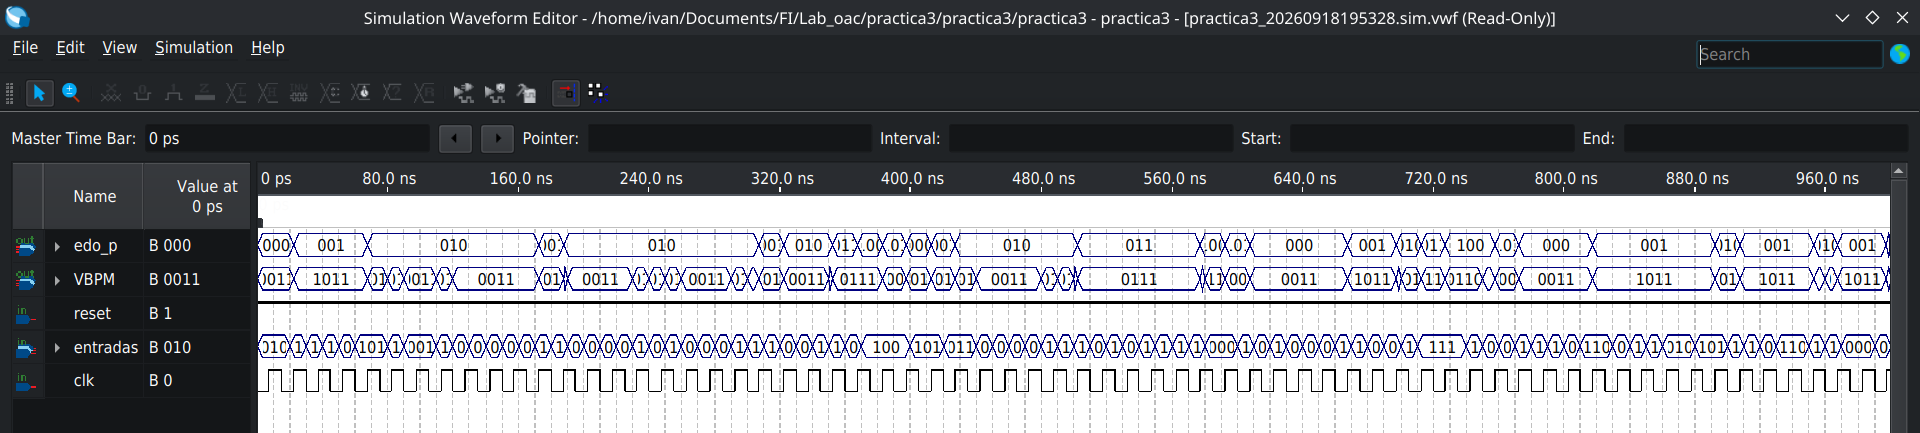
\includegraphics[width=\linewidth]{simulacion_1.png}
\caption{Primera Parte de la Simulación  en Quartus.}
\label{fig:simulacion-1}
\end{figure}

La Figura[\ref{fig:simulacion-2}] permite observar la relación temporal entre las señales. La palabra de la ROM, la entrada seleccionada y \texttt{Qsel} forman una ruta combinacional, de forma que  cuando cambia la entrada que está siendo evaluada, pueden cambiar la liga y las salidas antes del siguiente flanco de reloj. Sin embargo, \texttt{edo\_presente} conserva su valor durante ese intervalo, ya que el registro sólo acepta la liga en el flanco ascendente. 

Cuando el estado se encuentra en $S_1$, un cambio de $B=0$ a $B=1$ cambia la selección de la palabra de \texttt{LF=011}, \texttt{SF=1010} a \texttt{LV=100}, \texttt{SV=1000}. El estado mostrado continúa siendo \texttt{001} hasta el siguiente flanco posteriormente el registro presenta \texttt{100}. Este comportamiento confirma que el multiplexor de liga y el multiplexor de salidas reciben la misma señal \texttt{Qsel}, evitando que se seleccione una transición de una rama y la salida de la otra.

En los estados $S_3$, $S_4$ y $S_5$ no existe una decisión en la carta ASM. La ROM coloca los mismos valores en las ramas falsa y verdadera, por lo que cualquier valor de \texttt{Qsel} produce el mismo resultado. En consecuencia, $S_3$ conduce a $S_0$ con salida \texttt{0111}, $S_4$ conduce a $S_3$ con salida \texttt{0011} y $S_5$ conduce a $S_4$ con salida \texttt{0010}. La repetición de ambas alternativas en la palabra de memoria implementa correctamente las transiciones incondicionales.

\begin{figure}[H]
\centering
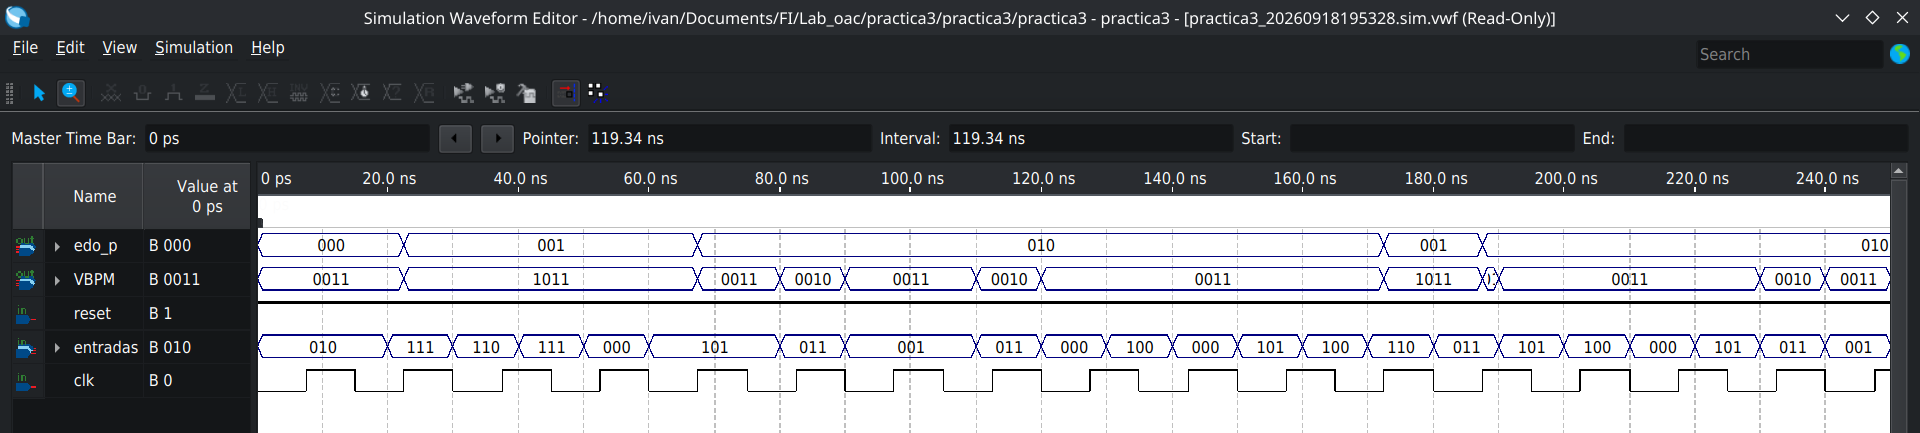
\includegraphics[width=\linewidth]{simulacion_2.png}
\caption{Detalle de las transiciones de estado y de las salidas durante la simulación.}
\label{fig:simulacion-2}
\end{figure}

Finalmente, en la Figura[\ref{fig:simulacion-3}] se observa el tramo en el que se mantienen las entradas en valores que permiten recorrer las ramas de la carta ASM. La secuencia de estados depende de la rama seleccionada en cada estado: desde $S_0$, $A=1$ lleva a $S_1$; en $S_1$, $B=0$ lleva a $S_3$ o $B=1$ lleva a $S_4$; desde $S_2$, $C=0$ lleva a $S_5$ y $C=1$ regresa a $S_0$. Las transiciones fijas completan los caminos restantes mediante $S_3\rightarrow S_0$, $S_4\rightarrow S_3$ y $S_5\rightarrow S_4$.

De esta manera, la simulación permite comprobar tres aspectos del diseño. Primero, el registro se reinicia correctamente en $S_0$. Segundo, cada estado direcciona la palabra correcta de la ROM y prueba la entrada indicada por \texttt{P1P0}. Tercero, la misma decisión \texttt{Qsel} selecciona de forma coherente la liga y las salidas, mientras que el reloj sincroniza el cambio de estado. 
\begin{figure}[H]
\centering
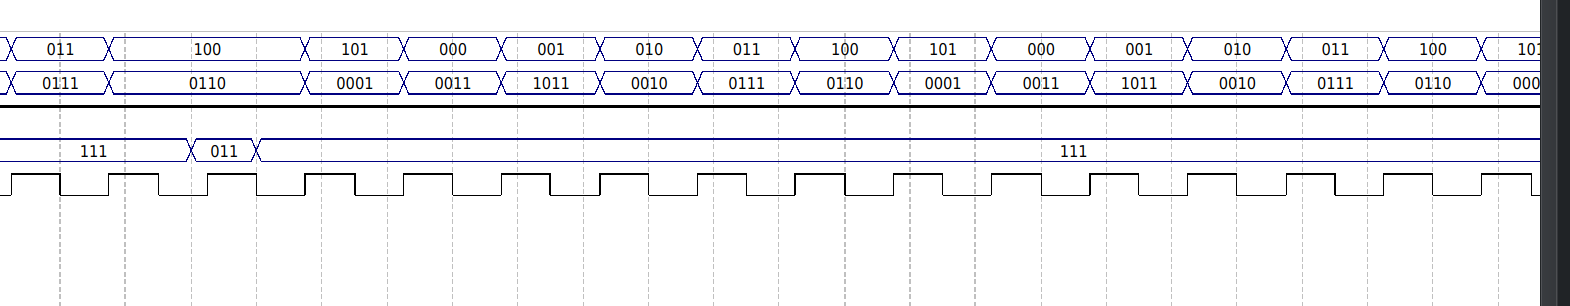
\includegraphics[width=\linewidth]{simulacion_3.png}
\caption{Parte final de la Simulación en Quartus, mostrando la secuencia de estados y salidas.}
\label{fig:simulacion-3}
\end{figure}

\section{Resultados en la tarjeta FPGA}

Las fotografías muestran la implementación sobre la tarjeta DE10-Lite. Los LEDs permiten observar el código de \texttt{edo\_presente} y el vector \texttt{salidas}. Se documentó $S_0$, las dos condiciones de $S_1$ y los estados restantes de la carta; con ello se contrastan las ramas dependientes de entrada y las transiciones incondicionales programadas en la ROM.

\begin{figure}[H]
\centering
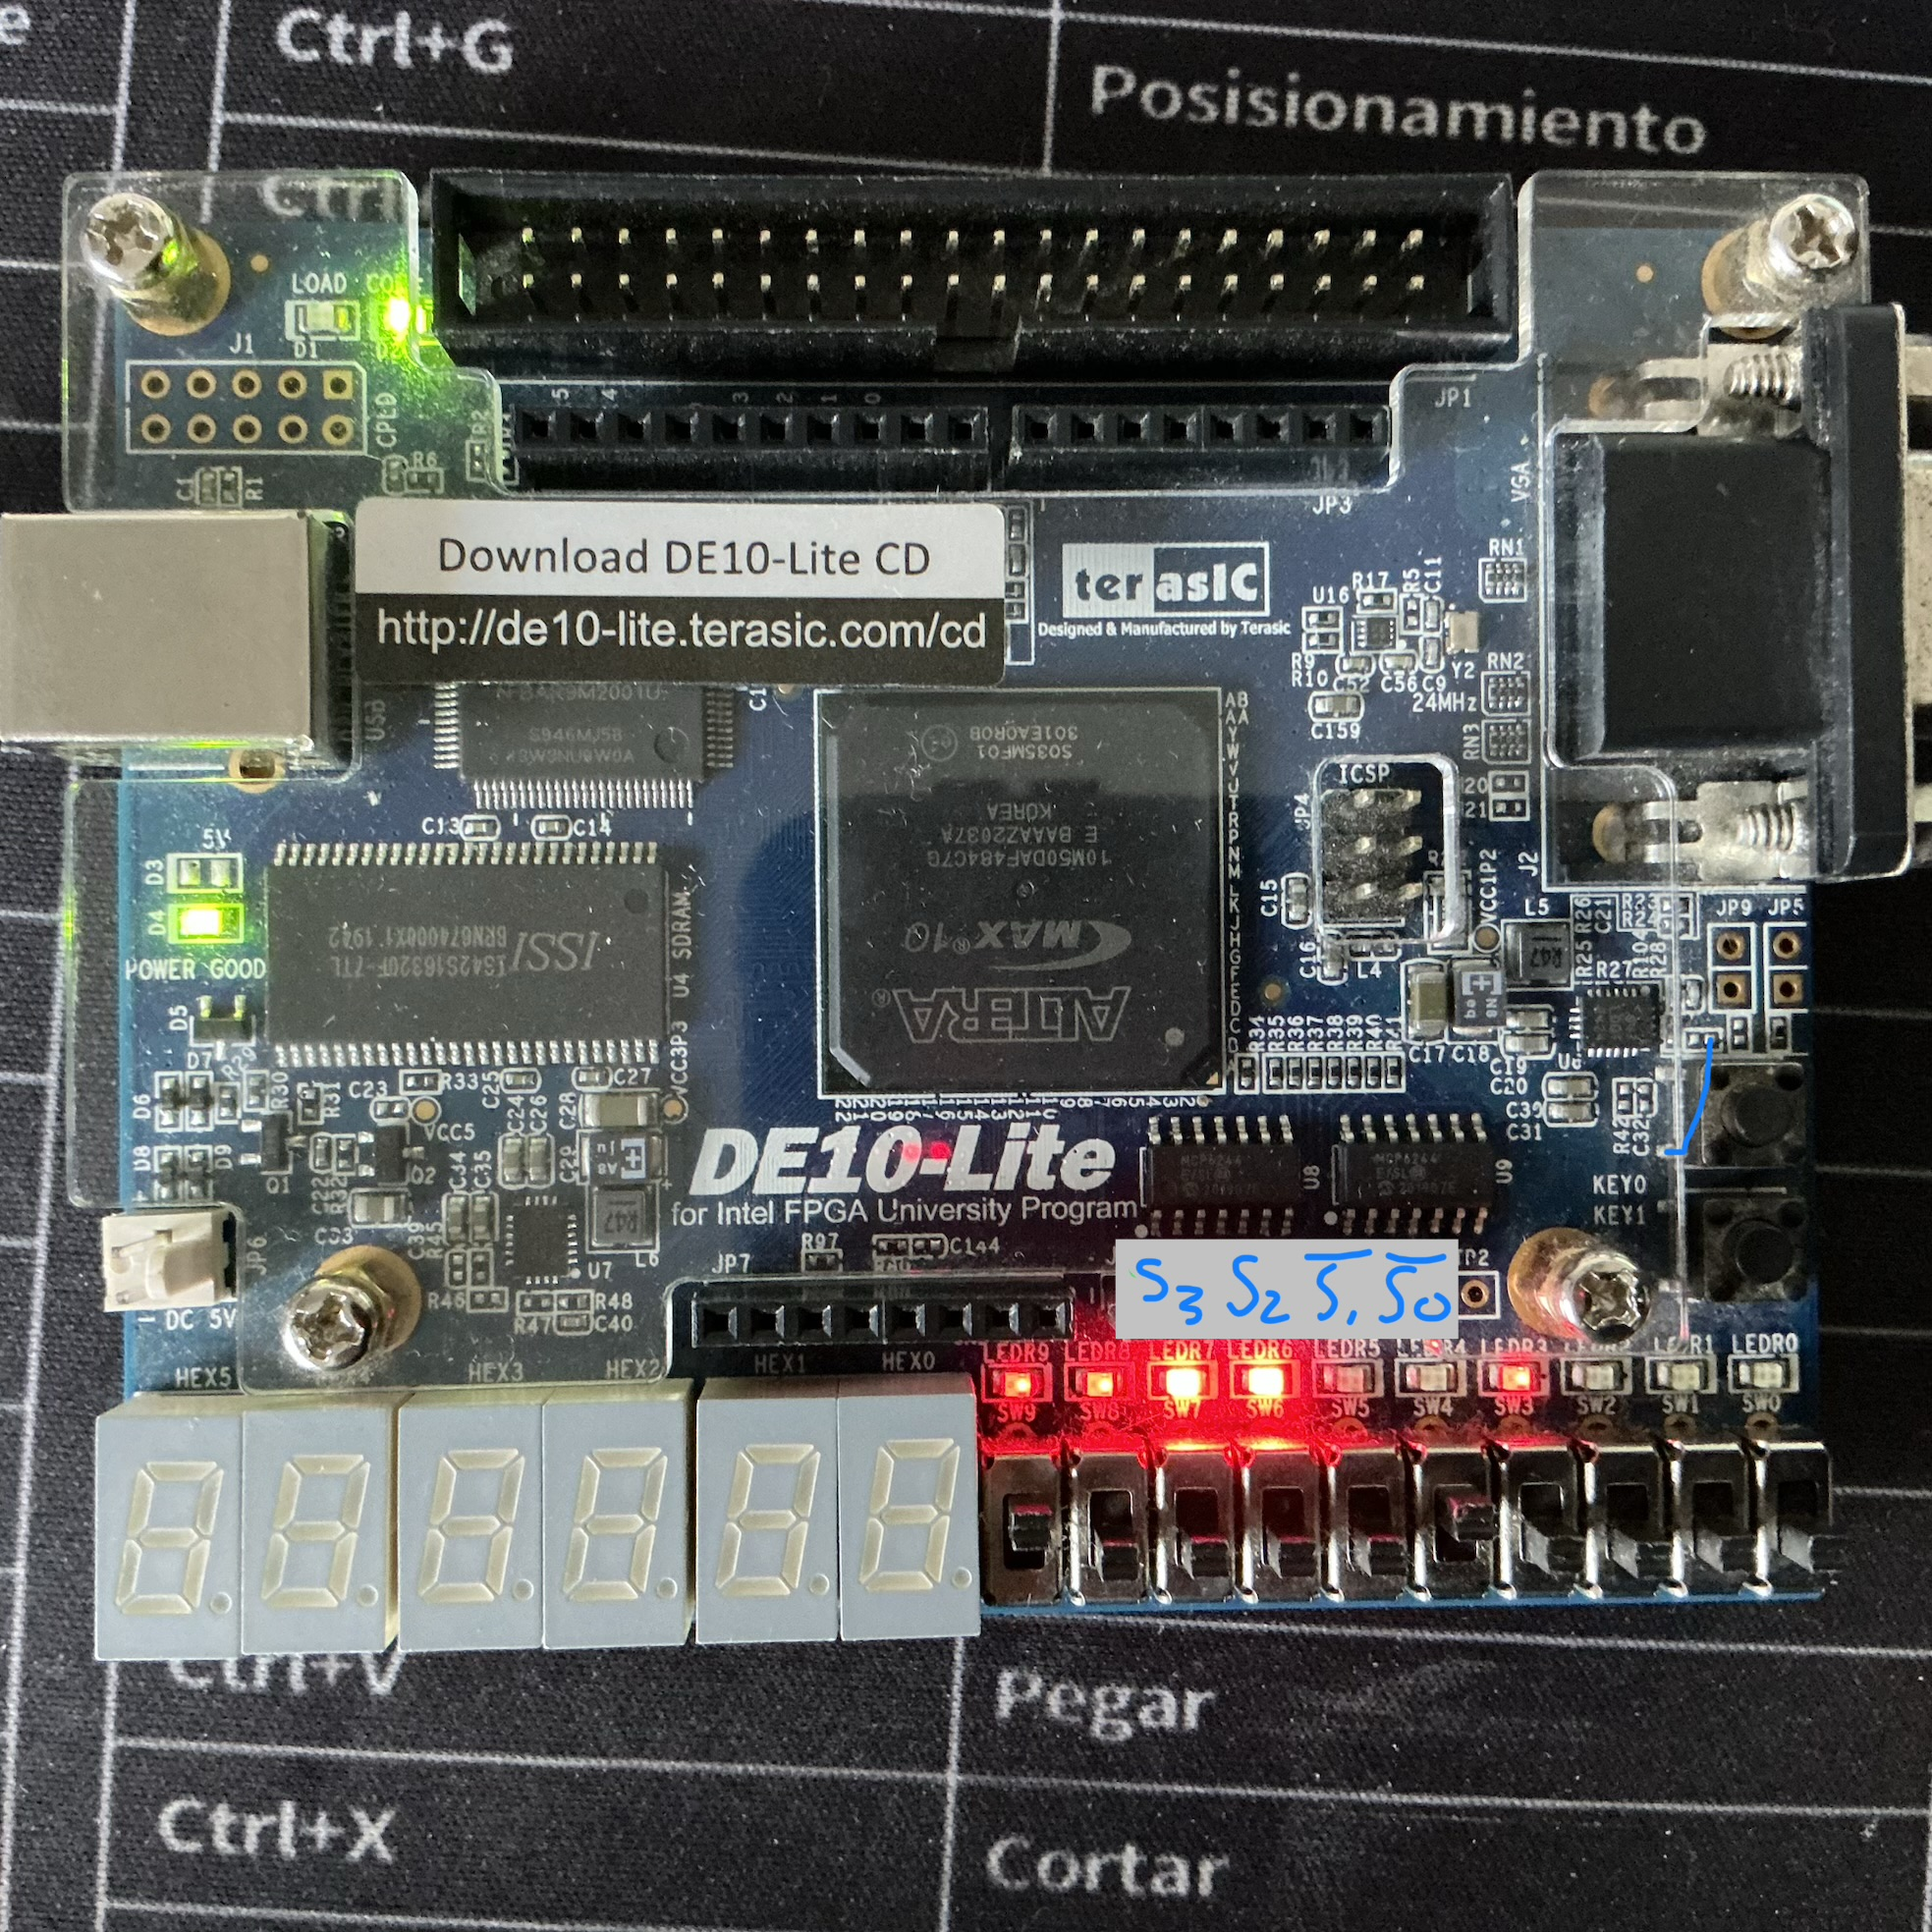
\includegraphics[width=0.44\linewidth]{est0.jpeg}
\caption{Evidencia en tarjeta del estado $S_0$, que prueba la entrada $A$.}
\label{fig:est0}
\end{figure}

\begin{figure}[H]
\centering
\begin{subfigure}[b]{0.44\linewidth}
  \centering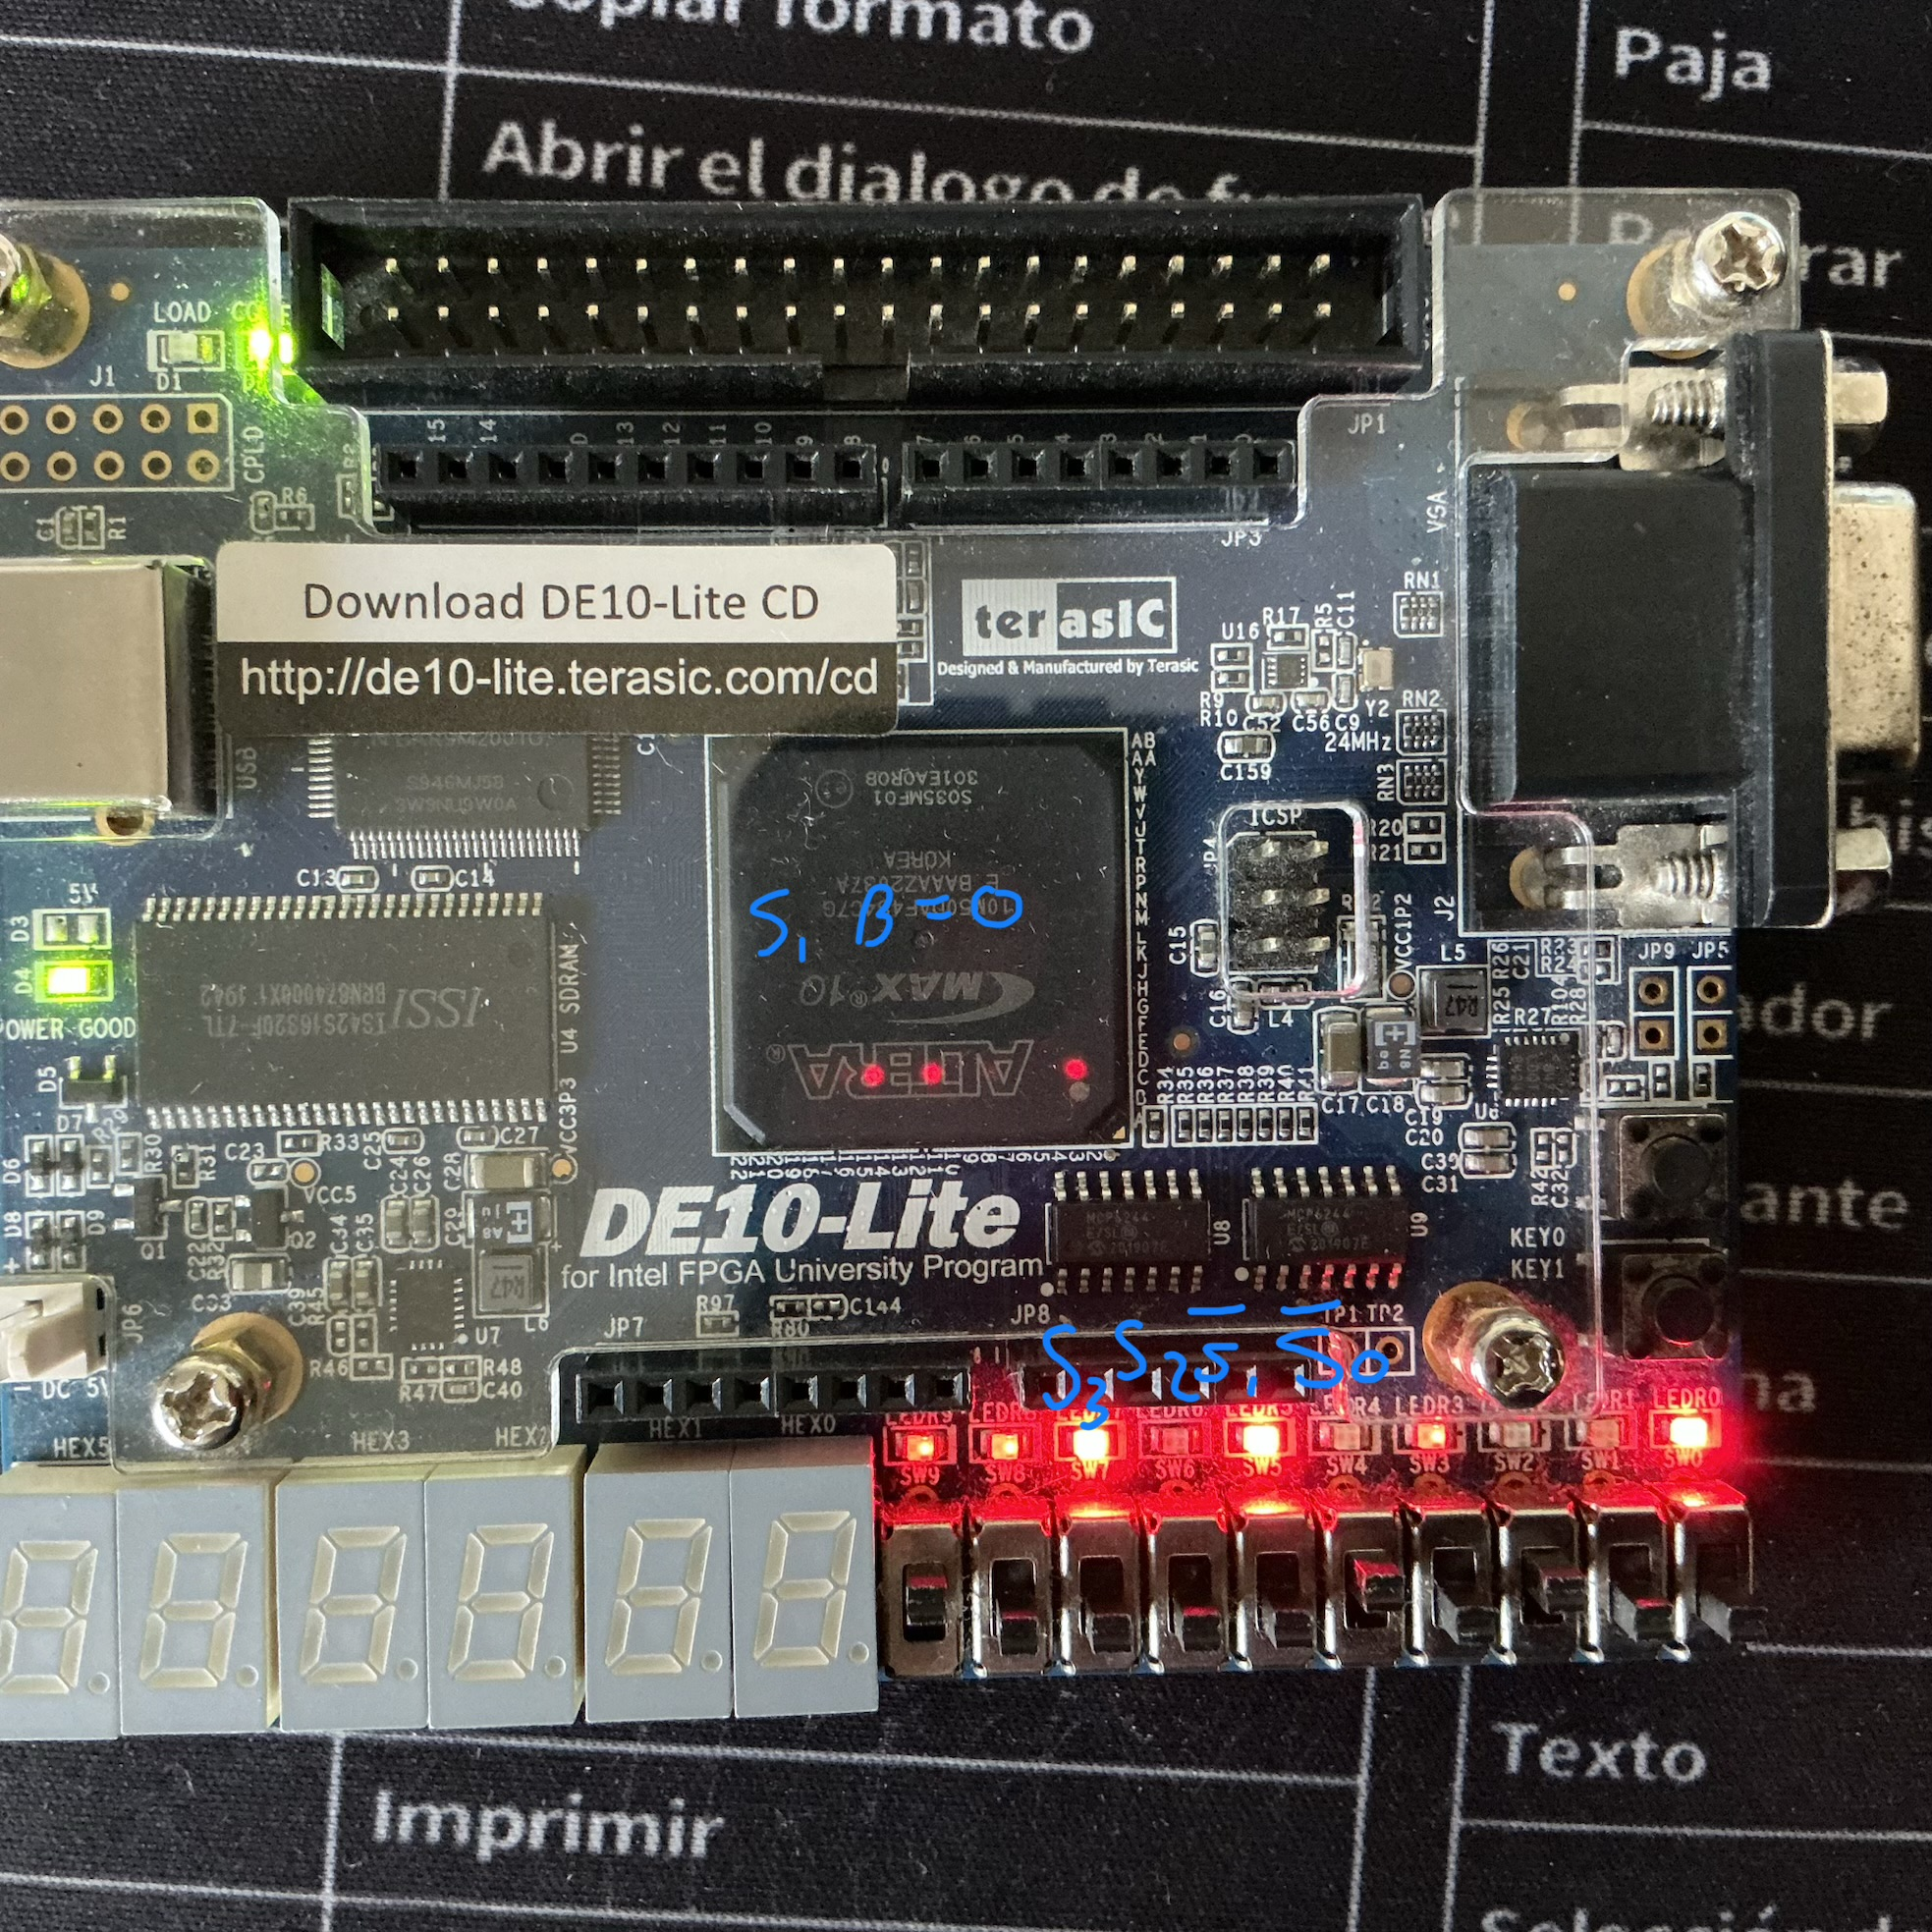
\includegraphics[width=\linewidth]{est1_b0.jpeg}
  \caption{$S_1$ con $B=0$: se selecciona la liga falsa hacia $S_3$.}
\end{subfigure}\hfill
\begin{subfigure}[b]{0.44\linewidth}
  \centering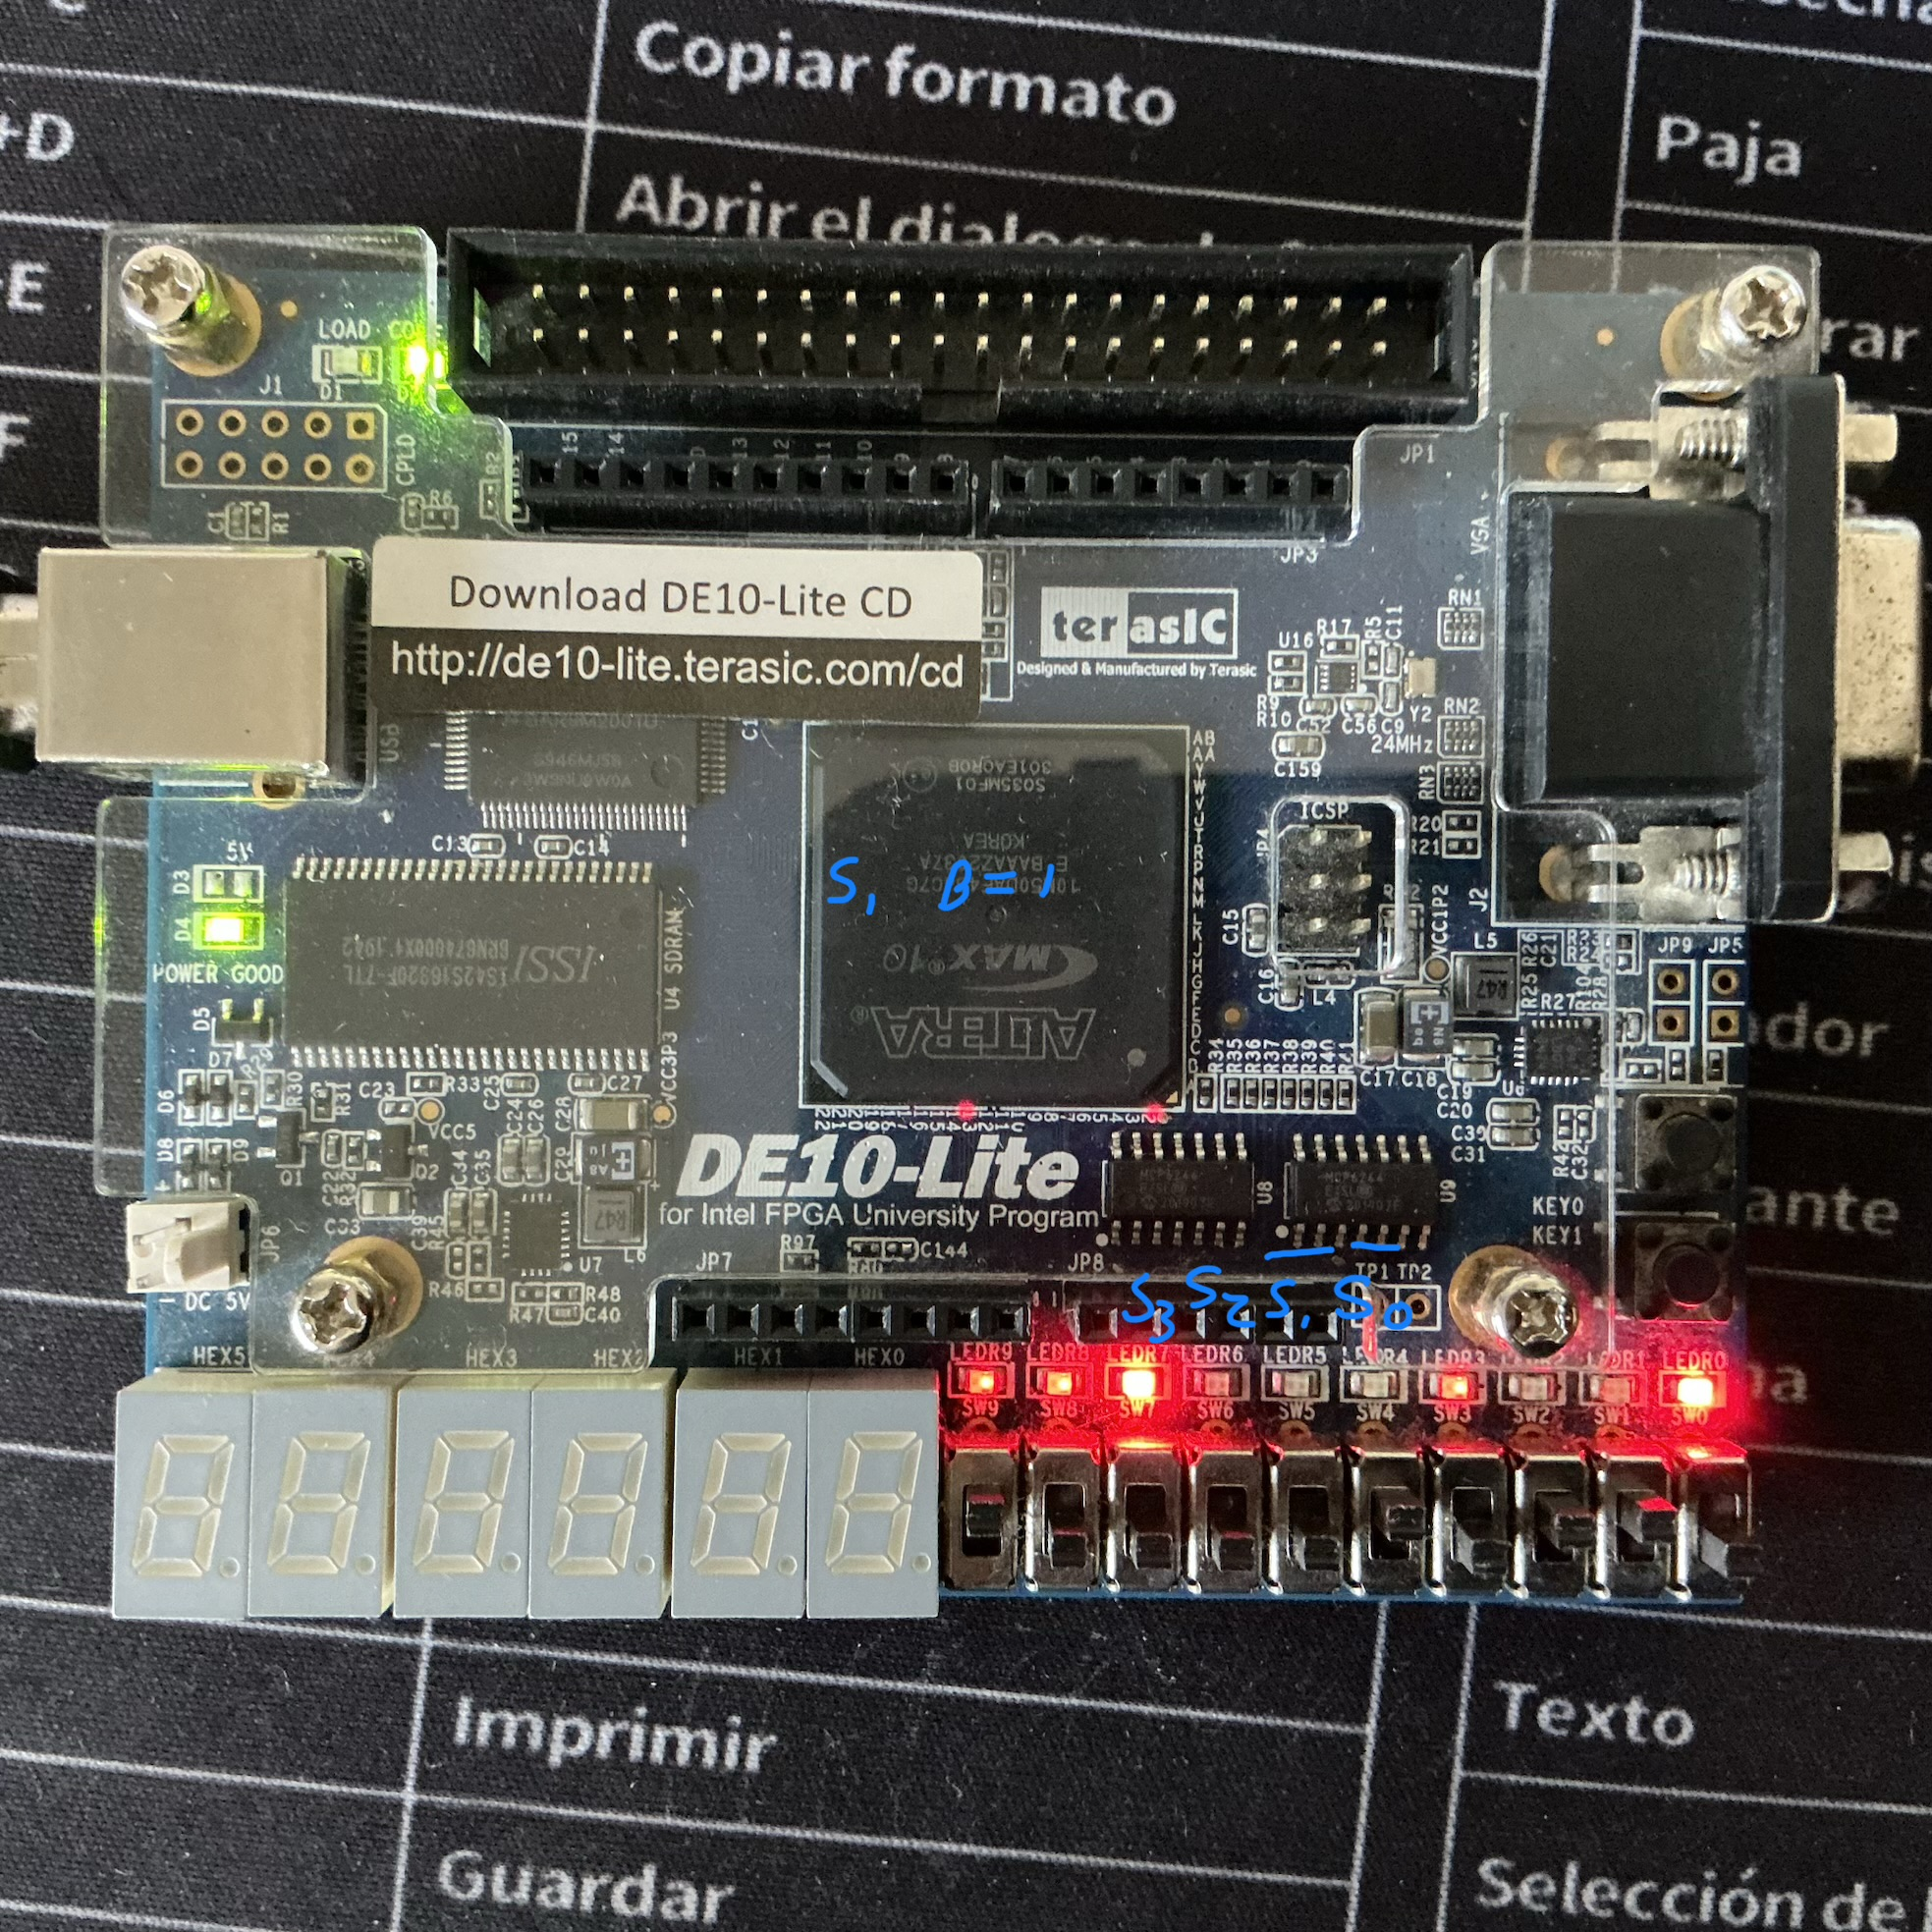
\includegraphics[width=\linewidth]{est1_b1.jpeg}
  \caption{$S_1$ con $B=1$: se selecciona la liga verdadera hacia $S_4$.}
\end{subfigure}
\caption{Verificación física de las dos ramas del estado $S_1$.}
\label{fig:est1}
\end{figure}

\begin{figure}[H]
\centering
\begin{subfigure}[b]{0.44\linewidth}
  \centering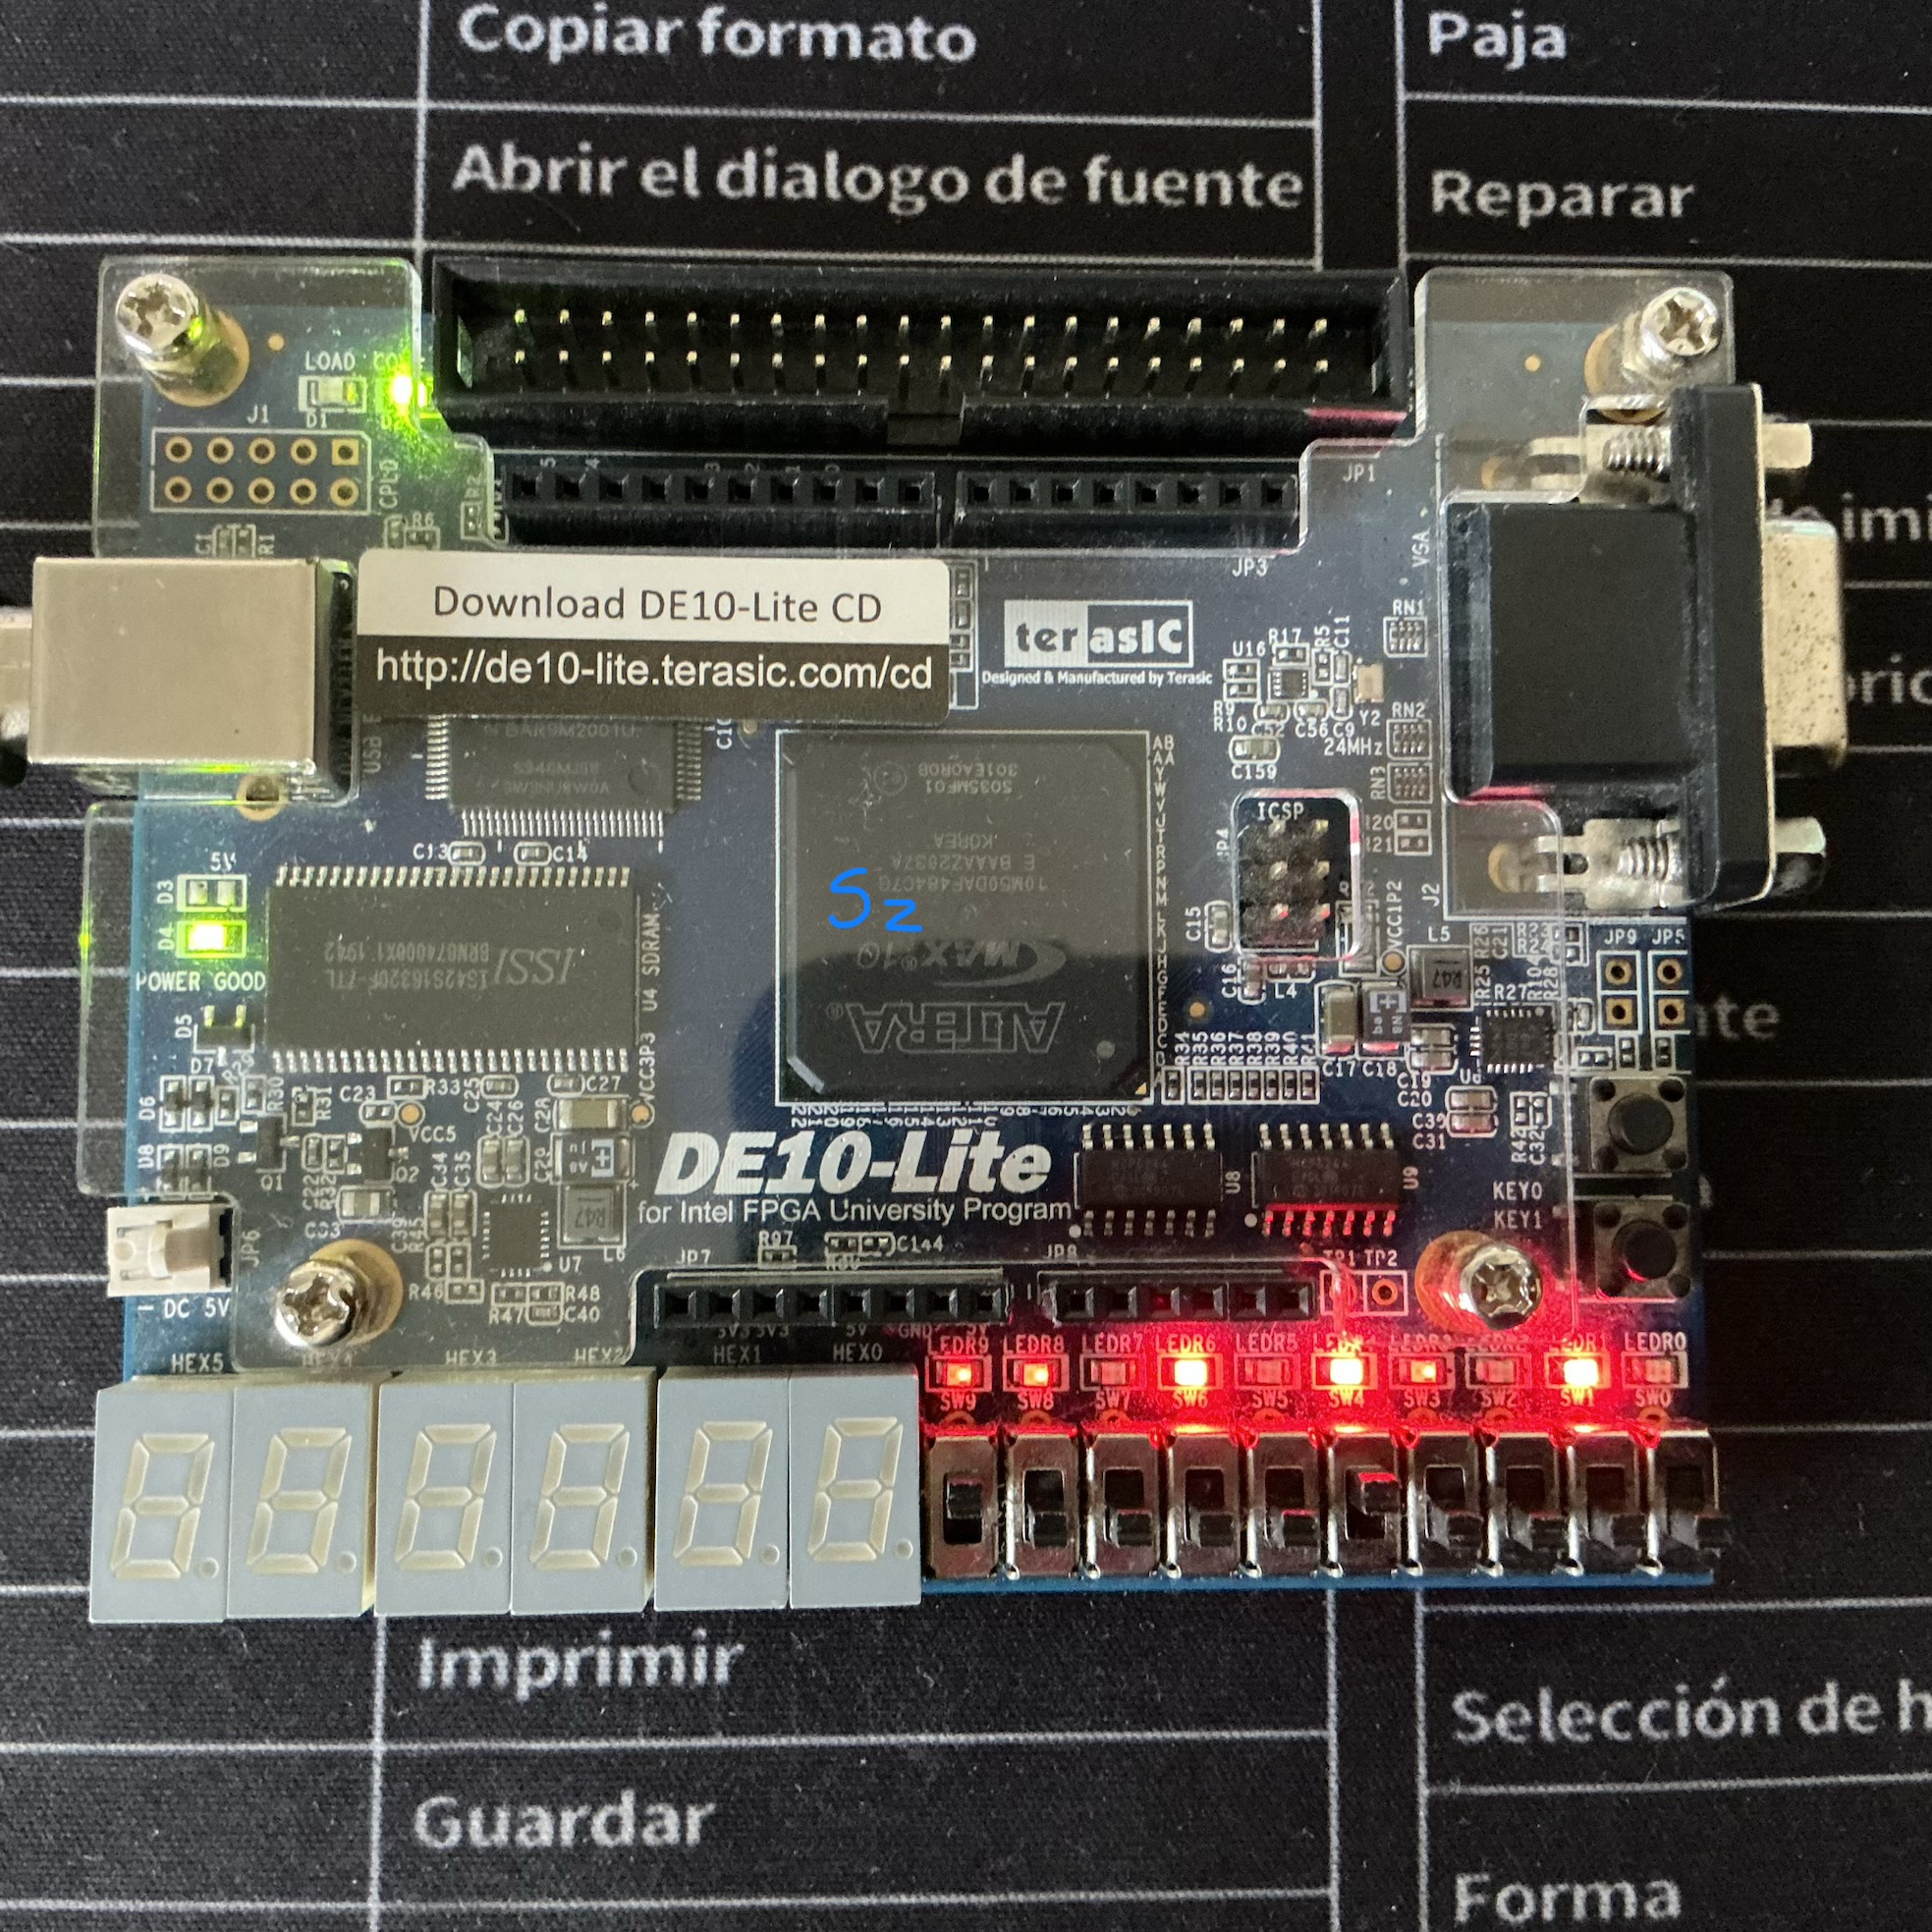
\includegraphics[width=\linewidth]{est2.jpeg}
  \caption{Estado $S_2$.}
\end{subfigure}\hfill
\begin{subfigure}[b]{0.44\linewidth}
  \centering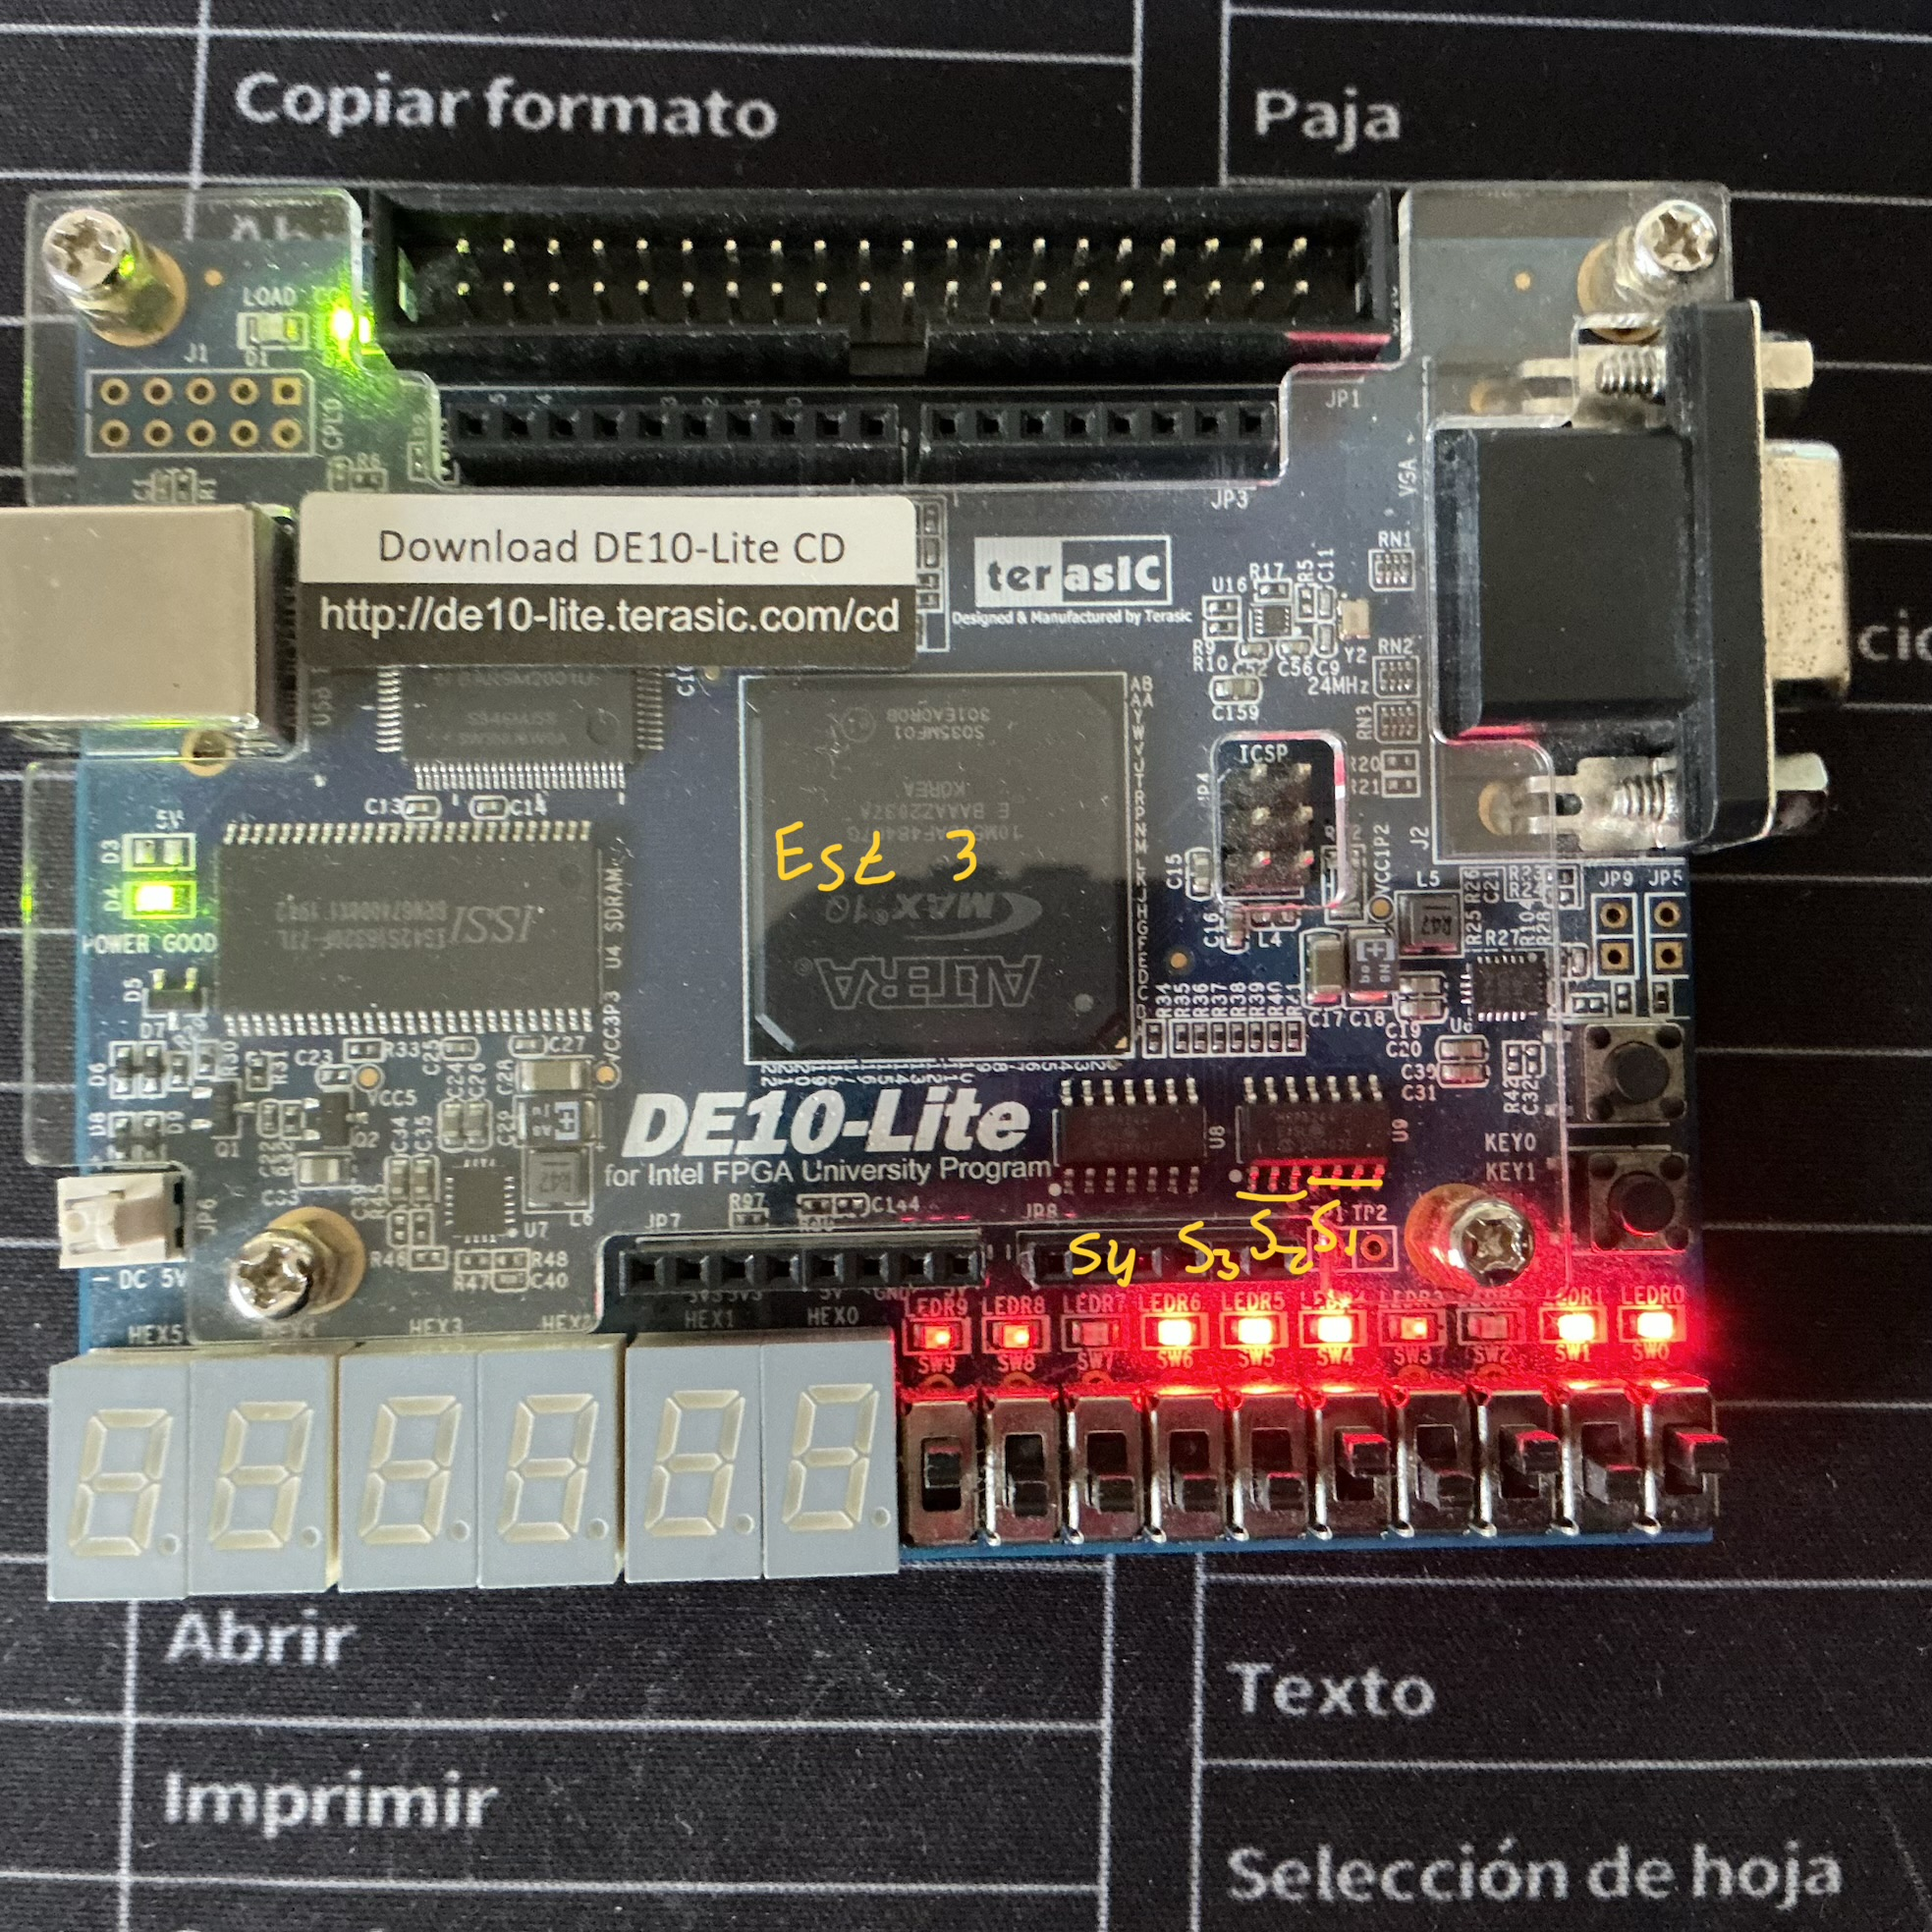
\includegraphics[width=\linewidth]{est3.jpeg}
  \caption{Estado $S_3$.}
\end{subfigure}\\[3mm]
\begin{subfigure}[b]{0.44\linewidth}
  \centering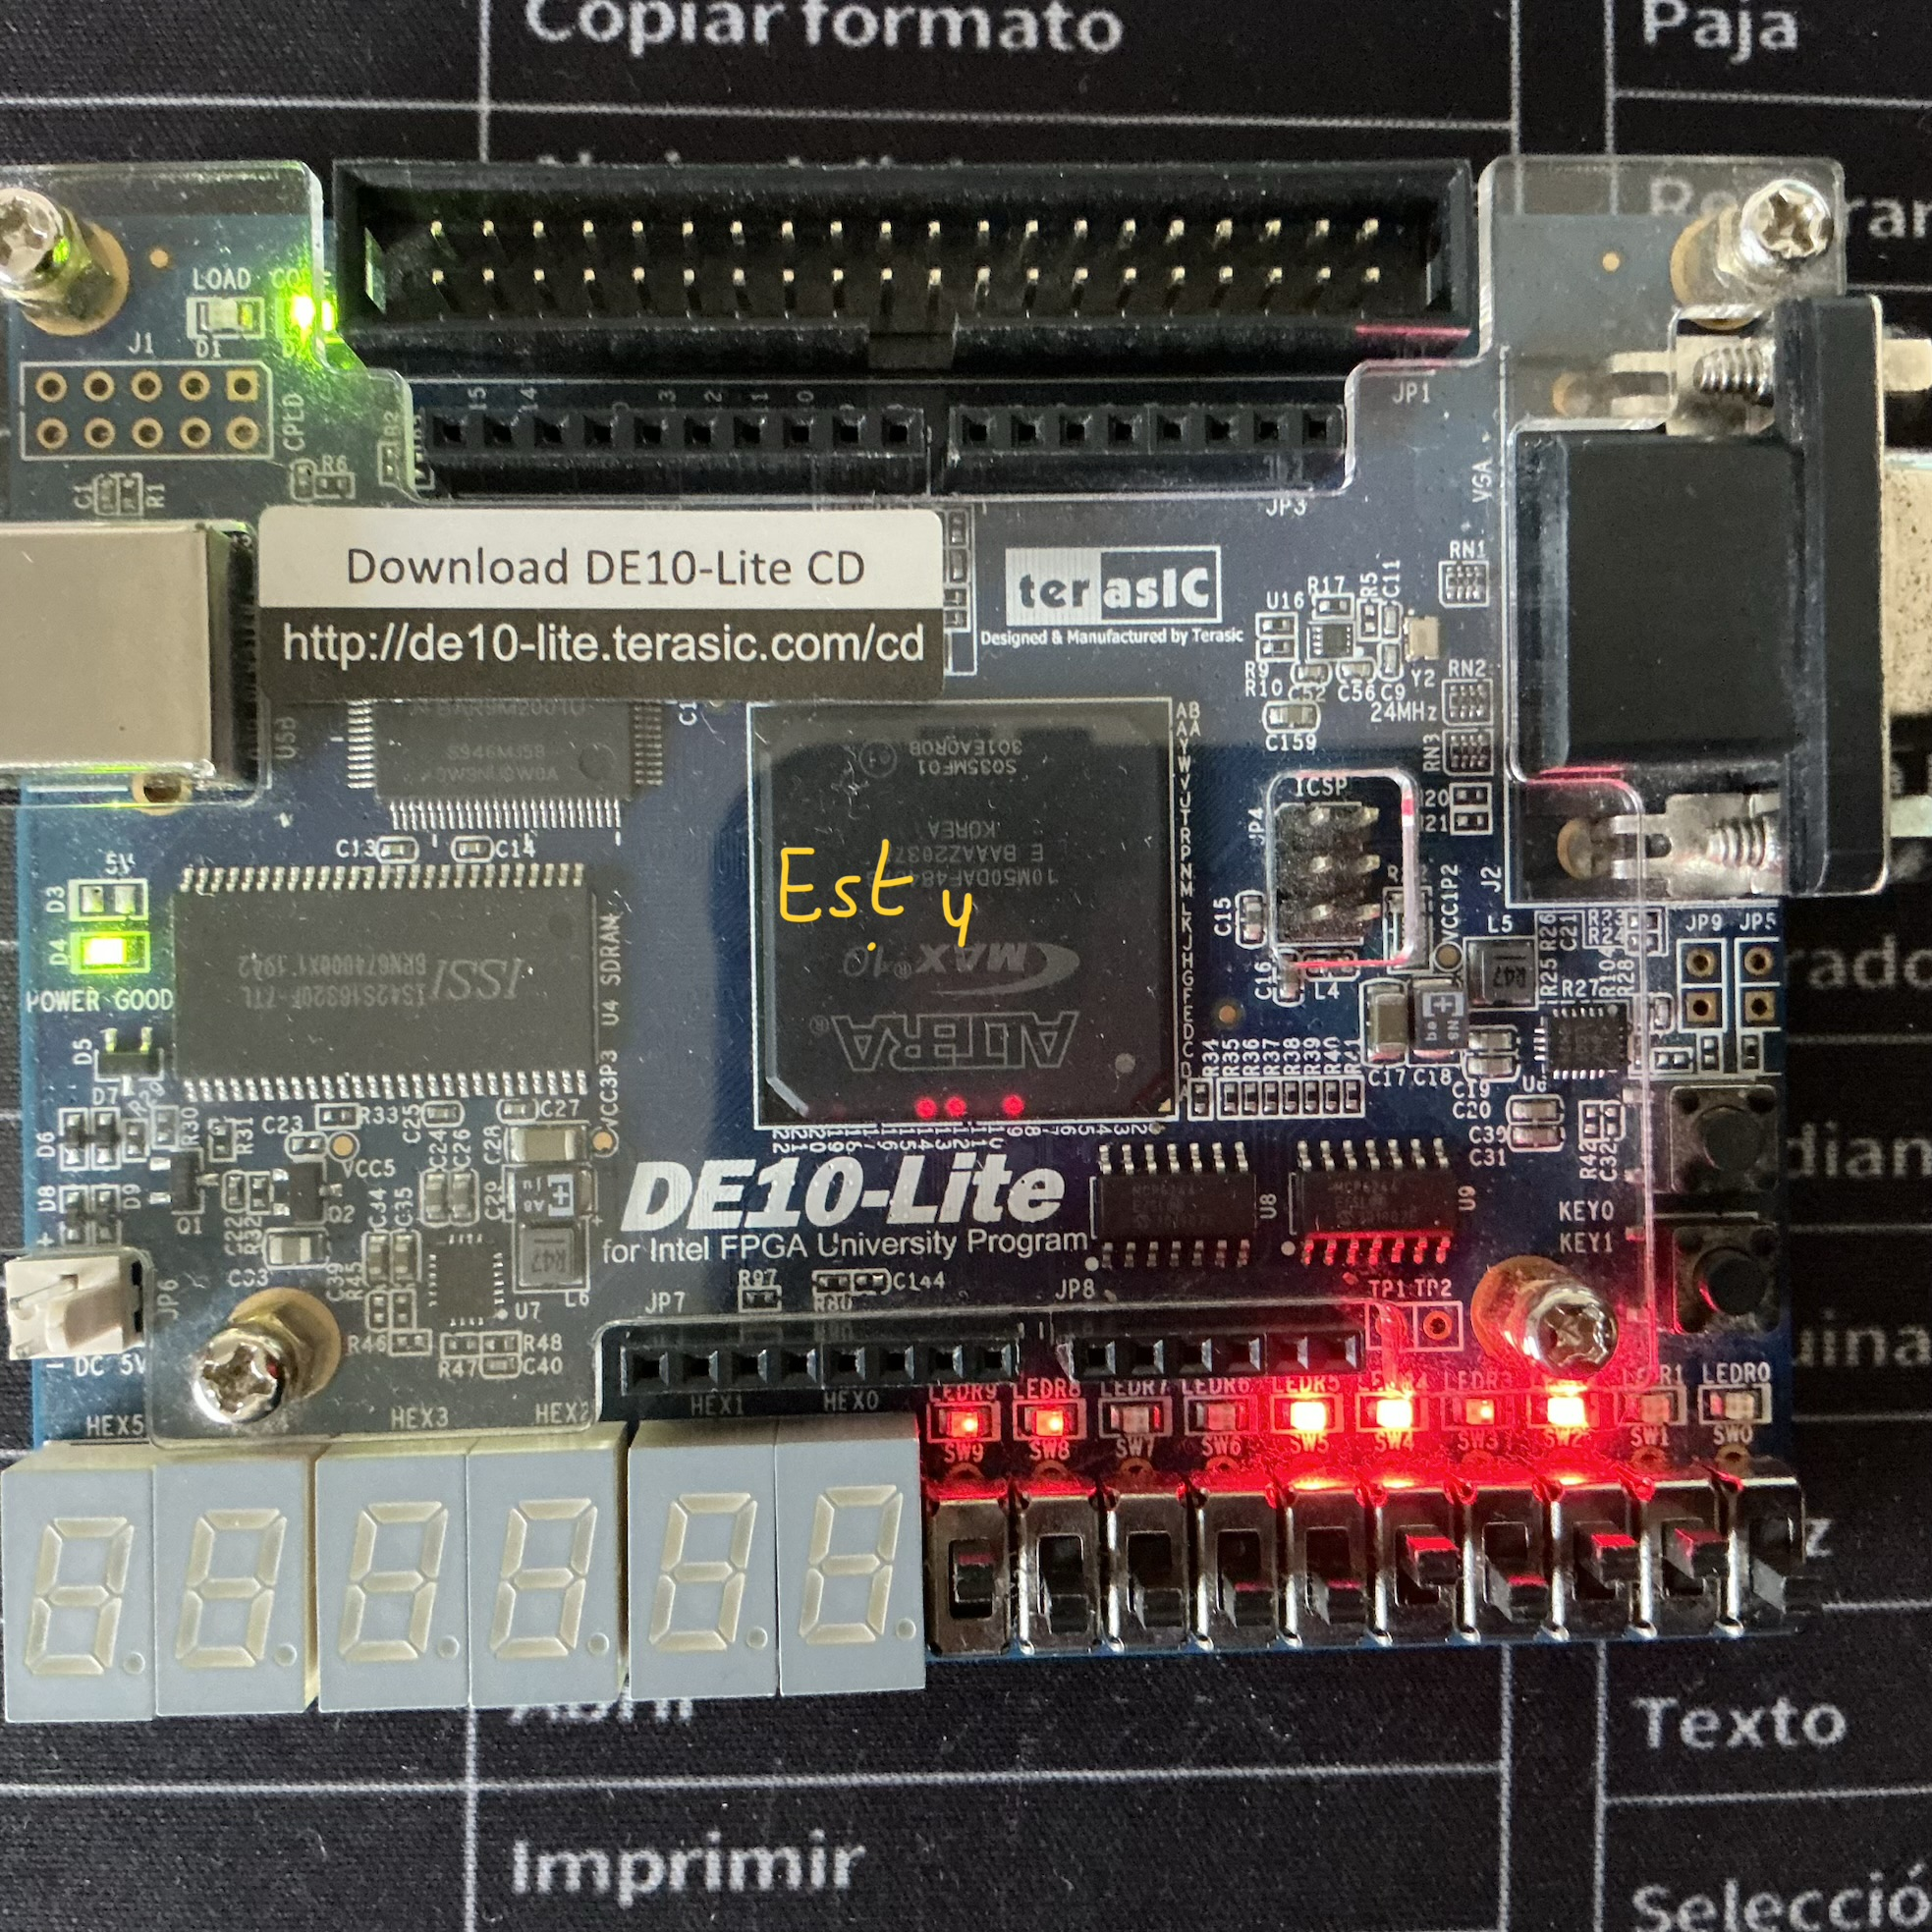
\includegraphics[width=\linewidth]{est4.jpeg}
  \caption{Estado $S_4$.}
\end{subfigure}\hfill
\begin{subfigure}[b]{0.44\linewidth}
  \centering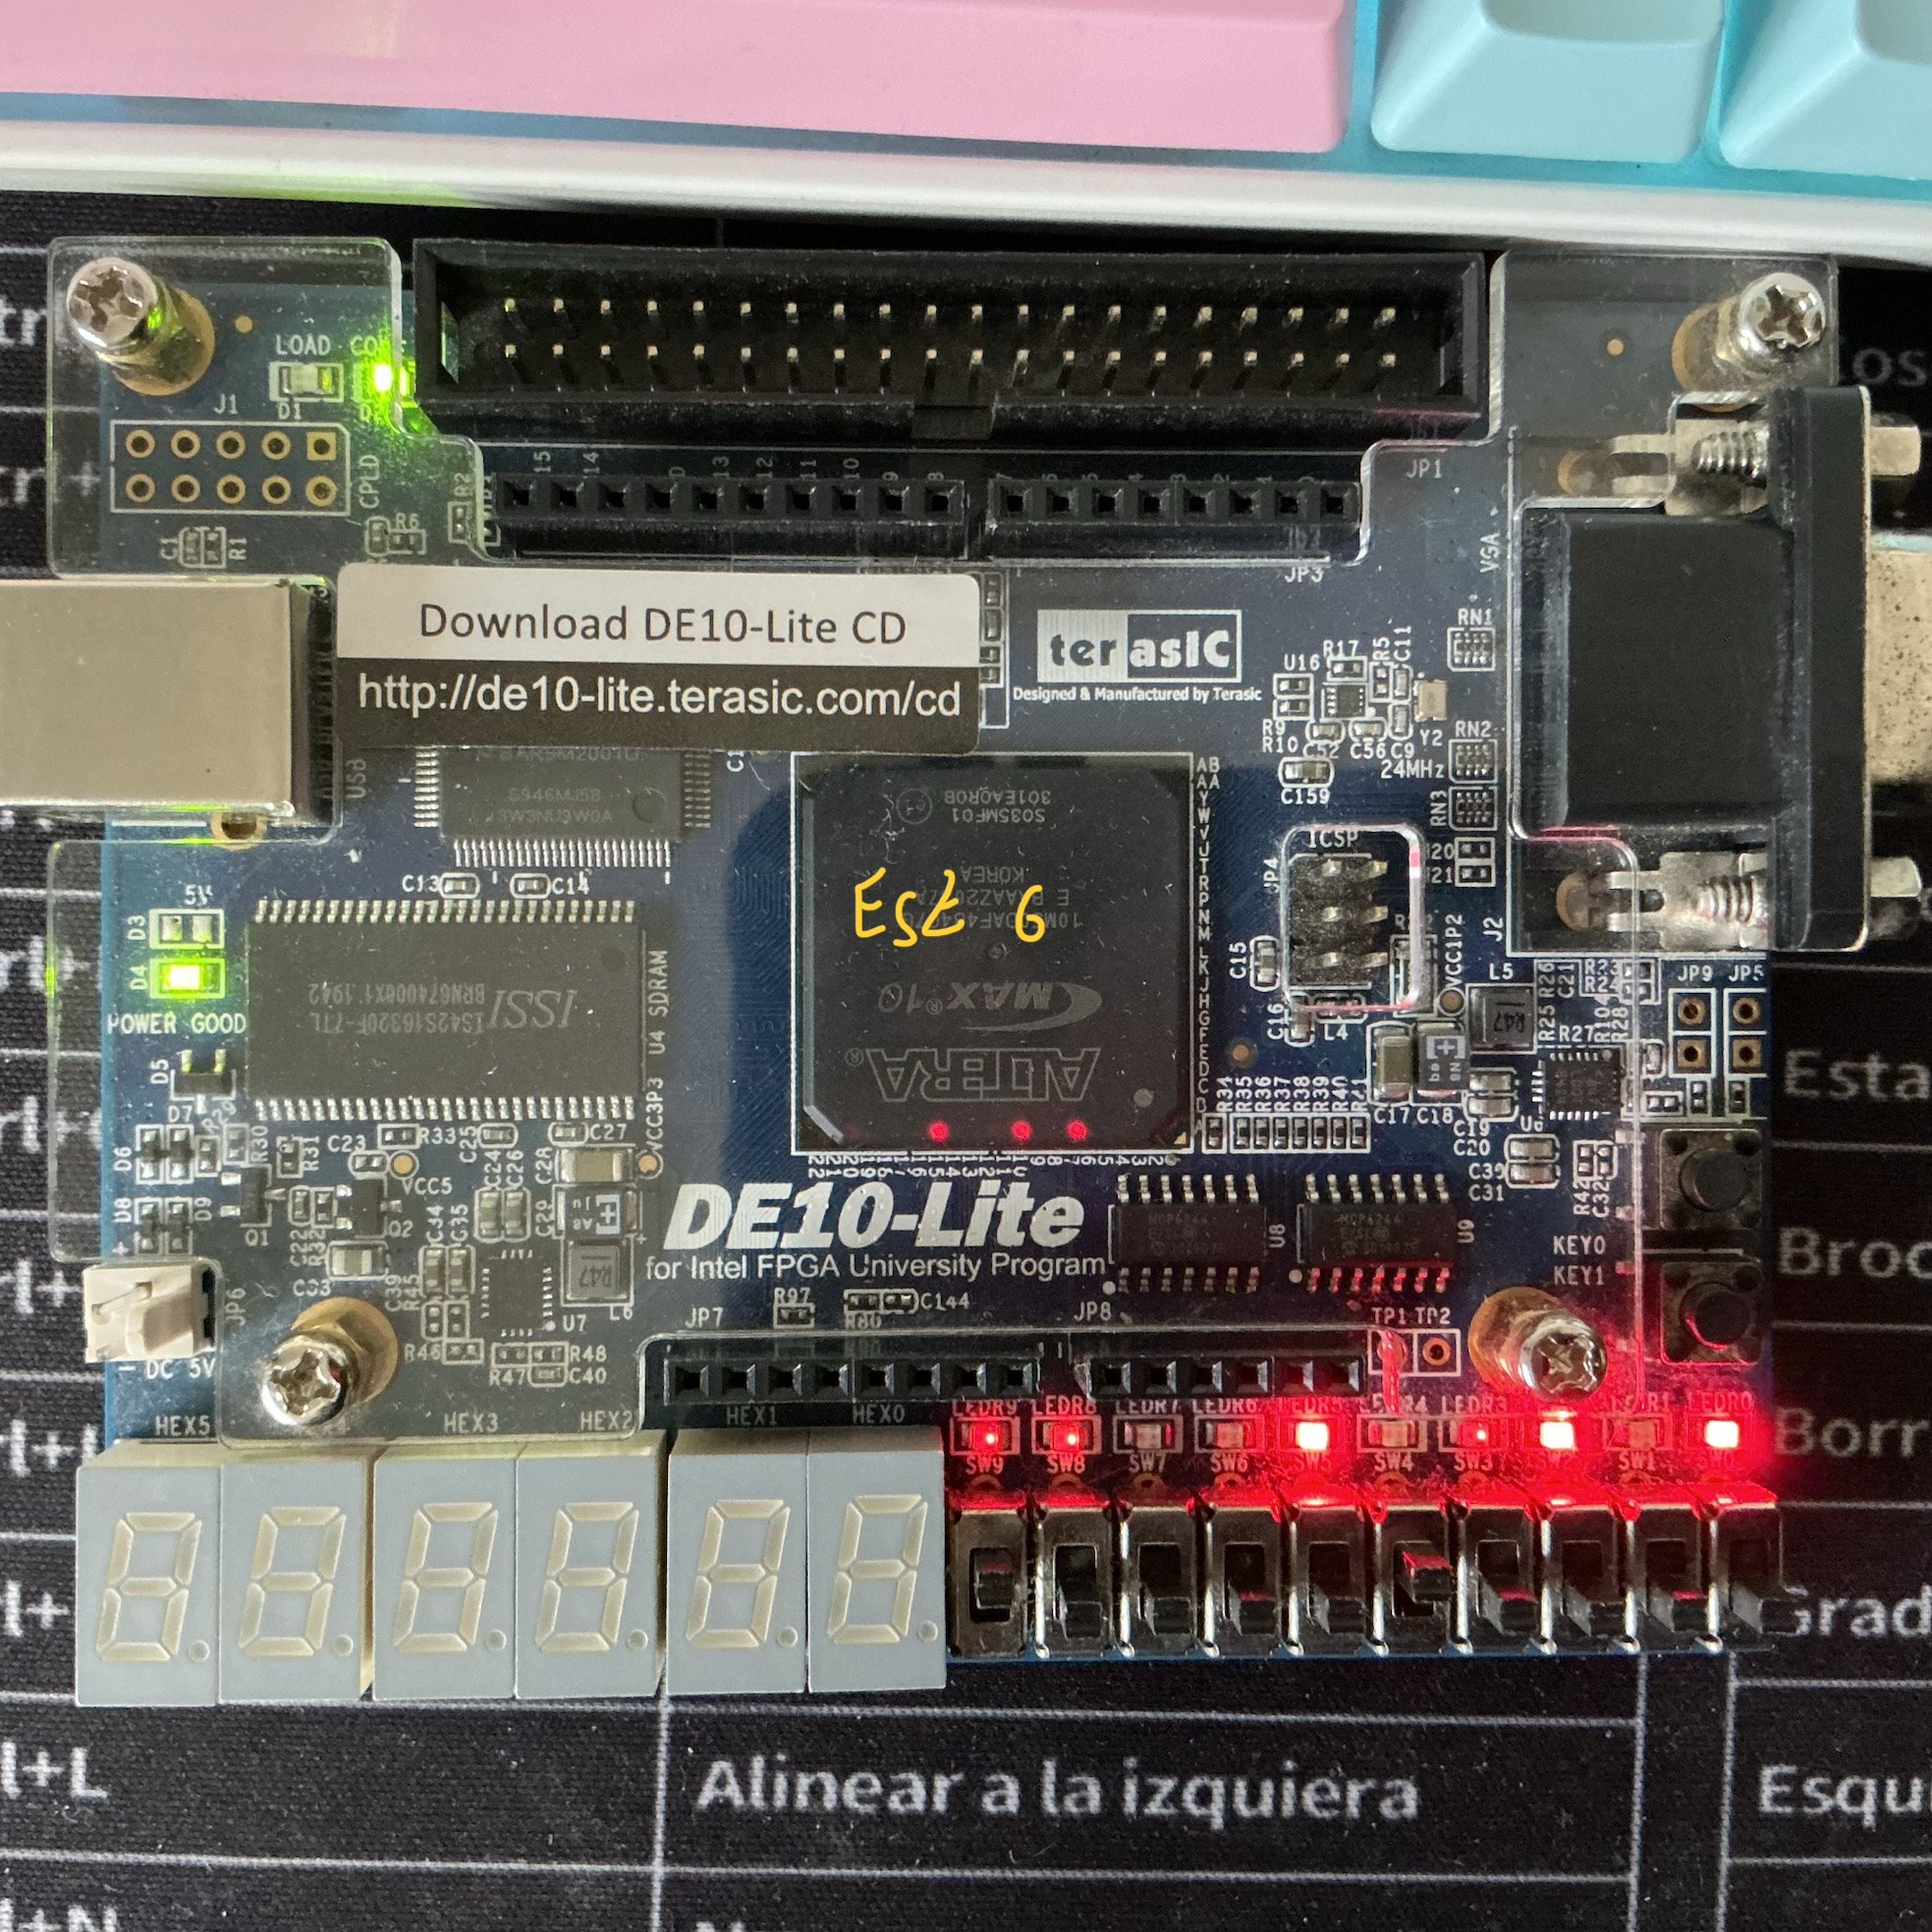
\includegraphics[width=\linewidth]{est5.jpeg}
  \caption{Estado $S_5$.}
\end{subfigure}
\caption{Evidencia en tarjeta de los estados $S_2$, $S_3$, $S_4$ y $S_5$.}
\label{fig:estados-2345}
\end{figure}

\clearpage
\section{Conclusión}

\paragraph{Percival Ulises Espinoza Matamoros.} Gracias a la realización de esta práctica pude comprender las diferencias entre el direccionamiento por trayectoria y el direccionamiento entrada-estado, así como la implementación del direccionamiento entrada-estado en lenguaje VHDL. Al implementar este tipo de direccionamiento, se puede observar cómo una sola palabra de memoria puede contener tanto la decisión que se evalúa como las dos posibles respuestas del sistema, esto se pudo visualizar de manera más clara en la implementacición física en la FPGA, así como las transiciones de estado en la simulación.

\paragraph{Oscar Iván Montiel Juárez.} En esta práctica aplicamos los conceptos vistos en teoría sobre máquinas de estados, codificación binaria, memorias ROM y multiplexores. Al implementar el método en VHDL y observarlo en la tarjeta FPGA, se comprendió cómo una palabra de memoria puede contener tanto la decisión que se evalúa como las dos posibles respuestas del sistema.

\paragraph{Amy Valentina Veraza García.} La simulación y las pruebas físicas permitieron verificar el funcionamiento de las ramas condicionadas por $A$, $B$ y $C$, así como los estados de transición fija. La comparación entre la tabla, los módulos VHDL y los LEDs de la tarjeta ayudó a validar el diseño completo.

\end{document}
